\documentclass{sfuthesis}
\title{Speed versus Accuracy in Neural Sequence Tagging for Natural Language Processing}
\thesistype{Thesis}
\author{Xinxin Kou}
\previousdegrees{%
	B.Sc. (Hons.), Dalhousie University, 2015}
\degree{Master of Science}
\discipline{Computing Science}
\department{School of Computing Science}
\faculty{Faculty of Applied Sciences}
\copyrightyear{2017}
\semester{Fall 2017}
\date{12 September 2017}

\keywords{Natural Language Processing; Sequence Tagging; Neural Networks}

\committee{%
	\chair{Dr.\ Arrvindh\ Shriraman}{Professor}
	\member{Dr.\ Anoop Sarkar}{Senior Supervisor\\Professor}
	\member{Dr.\ Fred Popowich}{Supervisor\\ Professor}
	\member{Dr.\ Jiannan Wang}{ Examiner \\
	Assistant Professor }
}
%   PACKAGES AND CUSTOMIZATIONS  %%%%%%%%%%%%%%%%%%%%%%%%%%%%%%%%%%%%%%%%%%%%%%
%
%   Add any packages or custom commands you need for your thesis here.
%   You don't need to call the following packages, which are already called in
%   the sfuthesis class file:
%
%   - appendix
%   - etoolbox
%   - fontenc
%   - geometry
%   - lmodern
%   - nowidow
%   - setspace
%   - tocloft
%
%   If you call one of the above packages (or one of their dependencies) with
%   options, you may get a ''Option clash'' LaTeX error. If you get this error,
%   you can fix it by removing your copy of \usepackage and passing the options
%   you need by adding
%
%       \PassOptionsToPackage{<options>}{<package>}
%
%   before \documentclass{sfuthesis}.
%
\usepackage{natbib}
\usepackage{apalike}
\usepackage{amsmath,amssymb,amsthm}
\usepackage[pdfborder={0 0 0}]{hyperref}
\usepackage{graphicx}
\usepackage{caption}
%\usepackage[numbers]{natbib}
\usepackage{algorithm}
\usepackage{algpseudocode}
\usepackage{array}
\usepackage{multirow}
\usepackage{underscore}
\usepackage{pgfplots}
\usepackage{subcaption}
\usepackage{graphicx}
\usepackage{makecell}
\pgfplotsset{width=10cm,compat=1.15}

\newcommand{\quotes}[1]{\textrm{``#1''}}
\newcommand{\ffa}{Feedforward-History}
\newcommand{\bia}{BiLSTM-Char}
\newcommand{\bib}{BiLSTM-CRF}
\newcommand{\ma}{Feedforward-Mention2Vec}
\newcommand{\mb}{BPE-Mention2Vec}
%   FRONTMATTER  %%%%%%%%%%%%%%%%%%%%%%%%%%%%%%%%%%%%%%%%%%%%%%%%%%%%%%%%%%%%%%
%
%   Title page, committee page, copyright declaration, abstract,
%   dedication, acknowledgements, table of contents, etc.
%

\begin{document}

\frontmatter
\maketitle{}
\makecommittee{}


\begin{abstract}
Sequence Tagging, including part of speech tagging, chunking and named entity recognition, is an important task in NLP. Recurrent neural network models such as Bidirectional LSTMs have produced impressive results on sequence tagging. In this work, we first present a Bidirectional LSTM neural network model for sequence tagging tasks. Then we show a simple and fast greedy sequence tagging system using a feedforward neural network. We compare the speed and accuracy between the Bidirectional LSTM model and the greedy feedforward model. In addition, we propose two new models based on Mention2Vec by \cite{stratos2016mention2vec}: \ma{} for named entity recognition and chunking, and \mb{} for part-of-speech tagging. \ma{} predicts tag boundaries and corresponding types separately. \mb{} uses the Byte Pair Encoding algorithm to segment words first and then predicts the part-of-speech tags for the subword spans. We carefully design the experiments to demonstrate the speed and accuracy trade-off in different models. The empirical results reveal that the greedy feedforward model can achieve comparable accuracy and faster speed than recurrent models for sequence tagging, and \ma{} is competitive with the fully structured BiLSTM model for named entity recognition while being more scalable in the number of named entity types.

\end{abstract}

\begin{dedication} % optional

To my beloved families who always support me and encourage me. 

\end{dedication}

\begin{acknowledgements} % optional

I would like to express my profound sense of gratitude to my supervisor Dr.\ Anoop Sarkar for introducing me to this research topic and providing his continuous support and valuable guidance throughout my graduate study. I can not imagine having a better advisor and mentor. In addition, I would like to express my sincere appreciation to Dr.\ Fred Popowich for his useful advice and feedback on this work, and Dr.\ Jiannan Wang for being my defence examiner and reading my thesis.

Thanks to all of my Natural Language Processing lab mates who helped me. I enjoy spending time with them. 


\end{acknowledgements}

\addtoToC{Table of Contents}\tableofcontents\clearpage
\addtoToC{List of Tables}\listoftables\clearpage
\addtoToC{List of Figures}\listoffigures





%   MAIN MATTER  %%%%%%%%%%%%%%%%%%%%%%%%%%%%%%%%%%%%%%%%%%%%%%%%%%%%%%%%%%%%%%
%
%   Start writing your thesis --- or start \include ing chapters --- here.
%

\mainmatter%

\chapter{Introduction}

In this chapter, we first describe sequence tagging tasks and introduce the motivation of this thesis. Then, we summarize our major contributions and describe the structure of the thesis.

\section{Sequence Tagging Task}

\subsection{Part-of-Speech Tagging (POS)}
Part-of-Speech Tagging (POS) is a basic sequence tagging task, which assigns each word with a unique tag that indicates its syntactic role, such as noun, adverb, verb, etc. Figure \ref{fig:pos-ex} illustrates a typical POS task. 

\begin{figure}
  \centering
  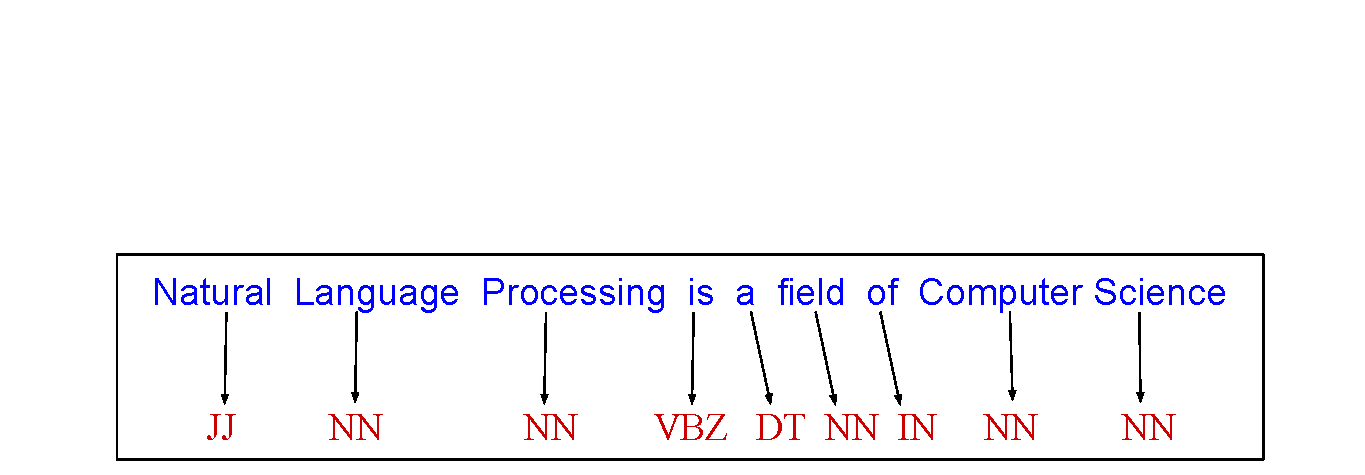
\includegraphics[scale=0.6]{posex.pdf}
 \caption{An example of POS}
  \label{fig:pos-ex}
\end{figure}

Most POS systems are evaluated on the English Penn TreeBank data set (\citeauthor{marcus1993building}, \citeyear{marcus1993building}), which contains 45 part-of-speech tags. The standard split uses section 1-18 of the Treebank for training, section 19-21 for tuning, and section 22-24 for testing (\citeauthor{toutanova2003feature}, \citeyear{toutanova2003feature}). The experimental data are summarized in Table \ref{table:my-dataset}. Many existing models are linear models, such as Maximum entropy Markov models (MEMMs) which obtain 96.46\% per word accuracy (\citeauthor{mccallum2000maximum}, \citeyear{mccallum2000maximum}); and the averaged perception discriminative model which obtains 97.11\% per word accuracy (\citeauthor{collins2002discriminative}, \citeyear{collins2002discriminative}). More recently, neural network models have been proposed to improve the state-of-the-art score. The Bidirectional LSTM network model proposed by \cite{huang2015bidirectional} reaches 97.55\% per word accuracy. \cite{ling2015finding} presents the compositional character-to-word LSTM model which reaches the state-of-the-art performance: 97.78\% per word accuracy. 

\begin{table}[]
\centering
\caption{Number of Words and Labels in Each Training, Validation and Test Section of Different Data Sets}
\label{table:my-dataset}
\begin{tabular}{|c|c|c|c|c|} \hline
      & Training  & Validation  & Test  & labels  \\ \hline
Penn Treebank   &950011 &40068 &56671 &45 \\\hline
CoNLL 2000   &211727 & N/A   &47377 &22   \\\hline
CoNLL 2003   &204567 &51578 &46666 &9     \\\hline
OntoNotes   &1088503 &147724 &152728 &18     \\\hline
\end{tabular}
\end{table}

\subsection{Named Entity Recognition (NER)}

\begin{figure}
  \centering
  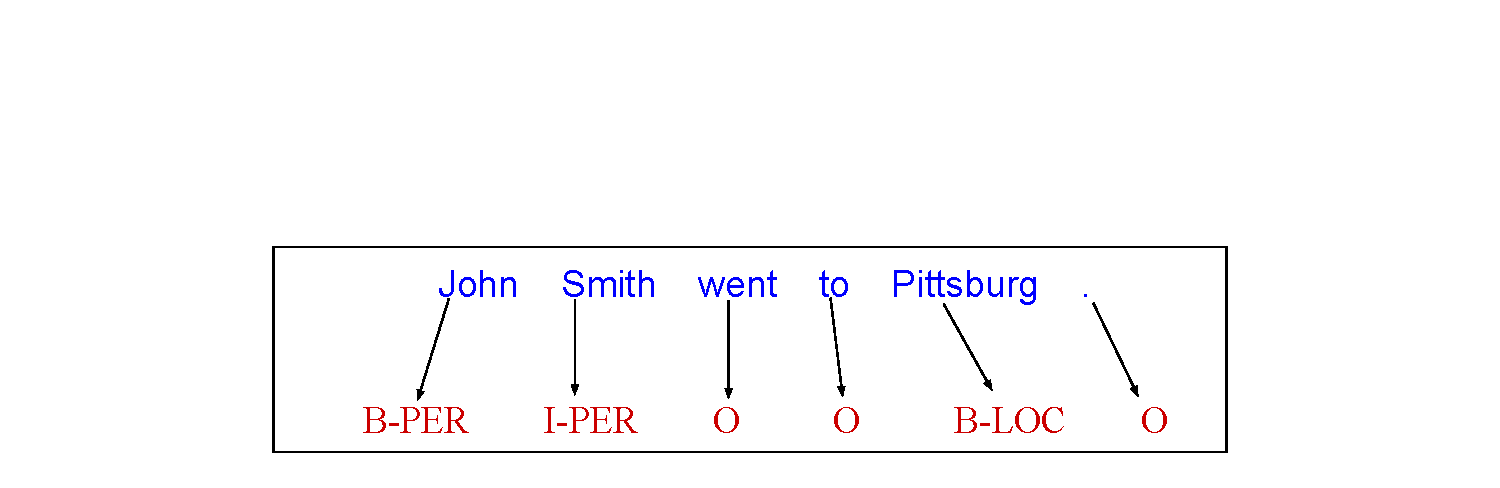
\includegraphics[scale=0.6]{nerex.pdf}
 \caption{An example of NER}
  \label{fig:ner-ex}
\end{figure}

Named Entity Recognition (NER) identifies expressions
that refer to named entities, such as people, places, organizations and others. The main difference between NER and POS is that each named entity label can span multiple words while each part-of-speech tag is only for one word. A popular convention in NER is to use the "IOB" label scheme (Inside, Outside, Beginning): if the word is the beginning of a named entity label, it is marked with B-label; if the word is inside a named entity label but not the first one, it is marked with I-label; if the token is outside the named entity, it is marked with "O". An example of NER is shown in Figure \ref{fig:ner-ex}. There are different numbers of named entity types in different NER tasks. For example, the shared task of CoNLL 2003 (\citeauthor{tjong2003introduction}, \citeyear{tjong2003introduction}) contains 4 types of named entities: locations (LOC), persons (PER), organizations (ORG), and miscellaneous (MISC); and the OntoNotes English data set (\citeauthor{hovy2006ontonotes}, \citeyear{hovy2006ontonotes}) contains 18 types of named entities shown in Table \ref{table:ontonotes-type}. The predefined training, development, and testing split of the data sets are shown in Table ~\ref{table:my-dataset}.

\begin{table}[]
\centering
\caption{Name Entity Types in OntoNotes}
\label{table:ontonotes-type}
\begin{tabular}{|c|c|} \hline
Types  & Named Entities  \\ \hline
PERSON & People, including fictional \\ \hline
NORP & Nationalities or religious or political groups \\\hline
FACILITY & Buildings, airports, highways, bridges, etc. \\ \hline
ORG & Companies, agencies, institutions \\ \hline
GPE & Countries, cities, states \\ \hline
LOC & Non-GPE locations, mountain ranges, bodies of water \\ \hline
PRODUCT & Vehicles, weapons, foods, etc. (Not services) \\ \hline
EVENT & Named hurricanes, battles, wars, sports events \\ \hline
WORK OF ART & Titles of books, songs \\ \hline
LAW & Named documents made into laws \\ \hline
LANGUAGE & Any named language  \\ \hline
DATE & Absolute or relative dates or period \\ \hline
TIME & Times smaller than a day  \\ \hline 
PERCENT & Percentage \\ \hline
MONEY & Monetary values, including unit \\ \hline
QUANTITY & Measurements, as of weight or distance \\ \hline
ORDINAL & First, Second, etc. \\ \hline
CARDINAL & Numerals that do not fall under another type \\ \hline
\end{tabular}
\end{table}

Most NER models are evaluated on CoNLL 2003 data set and are measured by the F1 score, which is the harmonic mean of precision and recall. 

\begin{equation}\label{eqn:softmax}
F_{1} = 2\times \dfrac{\textit{precision} \times \textit{recall}}{\textit{precision} + \textit{recall}}
\end{equation}

Since CoNLL 2003 has a relatively smaller amount of training data, most of the existing models make use of pretrained word embeddings along with the training data. A commonly used pretrained word embedding is GloVe (\citeauthor{pennington2014glove}, \citeyear{pennington2014glove}) which contains 40K words. The best system presented at the NER CoNLL 2003 challenge by \cite{florian2003named} obtains 88.76 F1 score. The model using Bidirectional LSTM by \cite{huang2015bidirectional} reaches 88.83 F1 score. Both of these two models use many external features along with a gazetteer\footnote{Gazetteers are language-specific knowledge resources}. \cite{lample2016neural} proposed two NER models with no external features or a gazetteer: the first one makes structured prediction using Bidirectional LSTM, Character Embeddings (\citeauthor{ling2015finding}, \citeyear{ling2015finding}) and Conditional Random Fields (CRF) (\citeauthor{lafferty2001conditional}, \citeyear{lafferty2001conditional}); and the second one uses a Shift-Reduce framework with Stack-LSTM (\citeauthor{dyer2015transition}, \citeyear{dyer2015transition}). The first model achieves 90.94 F1 score, while the second one performs slightly worse and achieves 90.33 F1 score. 

\subsection{Chunking}

Chunking is also known as shallow parsing which labels segments of a sentence with syntax tags, such as NP, VP, PP, etc.  An example of chunking is shown in Figure \ref{fig:ner-ex} The main difference between chunking and POS is that each chunking tag can span multiple words while each part-of-speech tag is only for one word. The "IOB" label scheme is used in chunking. An example of NER is shown in Figure \ref{fig:chunk-ex}. The best system using SVMs presented at the CoNLL 2000 challenge by \cite{Kudoh:2000:USV:1117601.1117635} obtains 93.48 F1 score. The current state-of-the-art score is 95.23 which is achieved by \cite{shen2005voting}. They use part-of-speech tags as features and a voting classifier for chunking. Recently, \cite{huang2015bidirectional} employs Bidirectional LSTM to solve chunking and achieved 94.46 F1 score with a number of hand-crafted features.
\begin{figure}
  \centering
  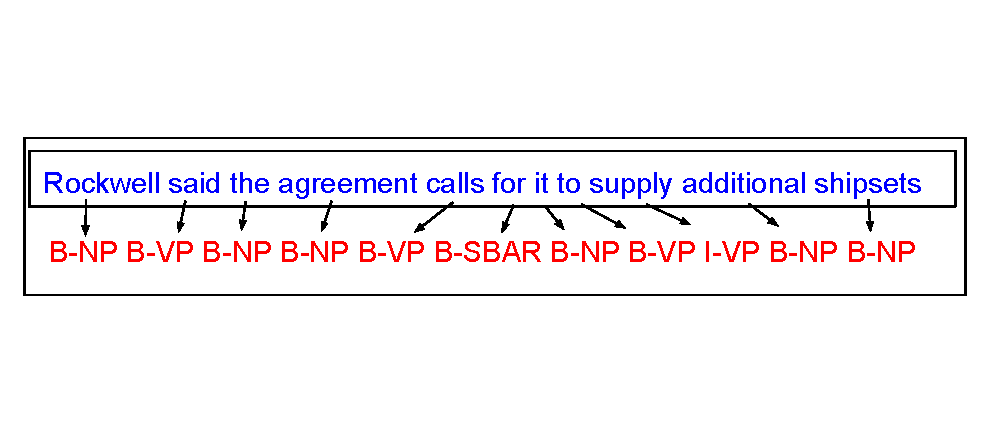
\includegraphics[scale=0.8]{Chunkingex.pdf}
 \caption{An example of Chunking}
  \label{fig:chunk-ex}
\end{figure}

\section{Motivation}
Recurrent Neural Networks (RNNs) have obtained impressive results in many NLP tasks, such as speech recognition (\citeauthor{graves2013speech}, \citeyear{graves2013speech}) and machine translation (\citeauthor{cho2014properties}, \citeyear{cho2014properties}).
Bidirectional Long Short Term Memory (BiLSTM) (\citeauthor{Hochreiter97longshort-term}, \citeyear{Hochreiter97longshort-term}; \citeauthor{graves2005framewise}, \citeyear{graves2005framewise}) is one of the RNN architectures that can maintain long-distance information from the past and future elements in an input sequence. Based on the existing work (POS system by \cite{ling2015finding} and NER system by \cite{lample2016neural}), state-of-the-art results on POS and NER can be obtained by using a BiLSTM network with Character Embeddings and Conditional Random Fields (CRF). Some work has also shown that feedforward neural networks can achieve comparable accuracy to recurrent models in tasks such as POS and Dependency Parsing (\citeauthor{andor2016globally}, \citeyear{andor2016globally}). One approach presented in this thesis is to employ a greedy transition system with a feedforward network to make independent classification decisions on each word. While the state-of-the-art model focuses on the sentence level and computes the score of every possible output sequence during decoding, the greedy system makes decisions on word level and can produce output sequence faster. However, the greedy system is limited when there are strong correlations between output labels. NER is one such task which has grammar constraints on output label sequences. For example, "I-PER" cannot follow "B-LOC" in NER. Next, we want to build a fast neural network model that can capture the dependencies among output tags.

Since the labels in Chunking and NER often span multiple tokens, most neural architectures for chunking and NER predict the boundaries and types of entities together using the "IOB" label scheme. Mention2Vec (\citeauthor{stratos2016mention2vec}, \citeyear{stratos2016mention2vec}) is proposed to address the natural segment-level representation by separating the NER task into boundary detection (I, O, B) and type prediction (PER, LOC, etc.). While Mention2Vec employs two BiLSTMs for each sub-task, we replace the BiLSTM layer for boundary detection with a feedforward network in order to obtain a simpler and faster model. This new model is denoted as Feedforward-Mention2Vec in this thesis.

We use Byte Pair Encoding (BPE) (\citeauthor{gage1994new}, \citeyear{gage1994new}) to deal with rare words in sentences for machine translation (\citeauthor{sennrich2015neural}, \citeyear{sennrich2015neural}), and we propose a new model combining BPE and Mention2Vec for POS, which is denoted as BPE-Mention2Vec in this thesis. We use BPE to segment the input words in the hope of capturing the orthographic evidence of the words without using spelling features (like prefixes and suffixes) or Character Embeddings. After we segment input words, POS becomes an NER-like task. Then, we can use Mention2Vec to solve the rest of the problem. Since boundaries of output tags are known in POS, we only need to use a BiLSTM network for type prediction in \mb.

There is increasing demand for faster sequence tagging systems to decode real time natural language data, such as Twitter, Facebook, Wikipedia, and even the web. Improving decoding speed will benefit many real world sequence tagging applications, but there is very little research into examining the decoding speed and accuracy relationship of different models. In this thesis, we will explore the speed and accuracy trade-off in different neural network models for sequence tagging. We re-implement many different types of feedforward models and BiLSTM models using Tensorflow (\citeauthor{abadi2016tensorflow}, \citeyear{abadi2016tensorflow}) and systematically compare the performance and decoding speed between them on sequence tagging tasks, such as POS and NER.

\section{Contribution}
The three main contributions of this thesis are:

\begin{enumerate}

\item  We implement the state-of-the-art sequence tagging model:BiLSTM with Character Embeddings and CRF, and we apply the fully structured BiLSTM model on all three sequence tagging tasks.

There is little work examining how the configurations of the fully structured BiLSTM model affect the decoding speed, such as whether the model is using Character Embeddings or the model is using CRF. We conduct experiments to compare the performance and decoding time of different configurations. 

\item We build a greedy tagging system with a feedforward neural network: \ffa. 

\ffa{} takes word features in context, spelling features, and previous tag features as input, and uses a feedforward neural network to predict tags word by word. There is little existing work measuring the decoding time using feedforward networks on sequence tagging, so we conduct experiments on sequence tagging and record the performance and decoding speed. To test the robustness of the feedforward networks, we also conduct experiments using a feedforward network with only word features, which also serves as the baseline. We compare the  feedforward model with the fully structured BiLSTM model and provide analysis on the results. 


\item Last but not least, we introduce two new neural architectures based on Mention2Vec: Feedforward-Mention2Vec for chunking and NER, and BPE-Mention2Vec for POS. 

Originally, Mention2Vec was designed for NER and used BiLSTMs to detect named entity boundaries and predict corresponding types separately. We propose Feedforward-Mention2Vec for Chunking and NER, in which we use a feedforward network with CRF to predict named entity boundaries instead of using a BiLSTM.  We denote this new model as \ma. We also adapt Mention2Vec for POS by combining Byte Pair Encoding (BPE) with BiLSTM in the model. BPE is used to segment the input words in our model, and it converts POS into a NER-like task. We denote this new model for POS as \mb. In BPE-Mention2Vec, we use a feedforward network to compute the hidden embeddings of the input segmented words. Since the boundaries of subword units are known, \mb{} does not need to predict the boundaries. It takes the hidden embeddings, tag boundaries, and a BiLSTM network to predict the actual POS tags. We benchmark these two multitask models against the state-of-the-art BiLSTM model on POS and NER. Since different NER tasks have different numbers of named entity types, the decoding time of a fully structured BiLSTM model grows quadratically in the number of types. In Mention2Vec and Feedforward-Mention2Vec, we only apply CRF on boundary labels ('I', 'O', 'B'), so the decoding time grows linearly in the number of types. To show the time difference on different NER tasks, we conduct the NER experiments on CoNLL 2003 which contains 4 different named entity types and OntoNotes which contains 18 different named entity types.

\end{enumerate}


\section{Overview}
The thesis is organized as follows:

In \textbf{Chapter 2} we present the fully structured BiLSTM model, which combines BiLSTM, Character Embeddings and CRF. We denote the fully structured model as the BiLSTM-CRF model. We explain the training and decoding process of BiLSTM-CRF, apply BiLSTM-CRF on POS and NER, and conduct experiments using three different configurations: BiLSTM with word features only, BiLSTM with Character Embeddings, and BiLSTM model with Character Embeddings and CRF.

In \textbf{Chapter 3}  we present a greedy tagging system using a feedforward neural network. Since the greed system takes into account the previous tag information and use a feedforward network to predict tags, we denote this model as \ffa. In order to show the robustness of this model, we also build a greedy feedforward model with only word features (denoted as Feedforward). We explain the training and decoding process of the feedforward models, describe the experiment design, and compare the performance and decoding time between feedforward models and BiLSTM models.


In \textbf{Chapter 4} we present two new multitask models based on Mention2Vec: Feedforward-Mention2Vec for Chunking and NER and BPE-Mention2Vec for POS. The intuition behind the multitask models is to capture the boundary information of tags and to reduce the decoding time. We explain the architectures of these two models and compare the performance and speed between multitask models and other models in this thesis.

In \textbf{Chapter 5} we discuss the empirical results from the previous chapters. We also analyze the trade-off between performance and speed in different neural network models.

In \textbf{Chapter 6} we summarize the contributions of this thesis and discuss ongoing and related future work.

\chapter{Bidirectional Long Short Term Memory Network Models}
In this chapter, we first describe Bidirectional Long Short Term Memory network (BiLSTM) and Character Embeddings. Then, we show the performance and decoding speed of BiLSTM models with different configurations on POS and NER.

\section{Model Description}
\subsection{Bidirectional Bidirectional Long Short Term Memory}

One major disadvantage of feedforward neural networks is that they only consider the context of the focused word instead of the whole sentence. Recurrent neural networks (RNNs) (\citeauthor{mikolov2010recurrent}, \citeyear{mikolov2010recurrent}) can keep the future and the past data persistent by using memory cells with loops in them. However, RNNs are biased towards the most recent data in practice. Long Short Term Memory Networks (LSTMs), special RNNs with Long Short Term memory cells  (\citeauthor{graves2005framewise}, \citeyear{graves2005framewise}), are designed to combat the bias problem. LSTMs learn long dependencies in a sequence with the help of Gates (\citeauthor{graves2005framewise}, \citeyear{graves2005framewise}). Gates control how much of the input information to pass to the next LSTM cell, and how much of the previous information to forget.

Given a sentence with $n$ words each of which is represented as a dense vector $x_i$, a LSTM makes use of $x_{1:n}$ to compute a forward representation $\overrightarrow {h_{i}}$ for the $i$th word. In general, computing a backward representation $\overleftarrow {h_{i}}$ would be useful for sequence tagging. Bidirectional LSTM (BiLSTM) is an extension to LSTM which takes into account both the past elements and the future elements in a sequence. A BiLSTM generates both $\overrightarrow {h_{i}}$ and $\overleftarrow {h_{i}}$ for the $i$th word in a sequence. The hidden embedding $h_{i}$ is the concatenation of $\overrightarrow {h_{i}}$ and $\overleftarrow {h_{i}}$. BiLSTM mapping is defined as $BiLSTM_{\theta}$:
$h_{i} = BiLSTM_{\theta}\left(x_{1:n}, i\right)$ where $\theta$ represents trainable parameters in BiLSTM.

 We can combine BiLSTM with CRF to make use of sentence level tag information. As in the Feedforward-CRF model, we introduce a transition matrix $T$ to keep the transition score from $y_{i}$ to $y_{i+1}$. Given an output sequence $Y$, the score of the output sequence is given by:

\begin{equation}
S\left( X|Y\right)=\sum _{i}^{n}T_{i,i+1}+\sum _{i}^{n}P_{i}
\end{equation}

We can use the dynamic programming algorithm to compute the transition matrix and find the optimal output tag sequence. Figure \ref{fig:bilstmcrf} illustrates the BiLSTM model with CRF on an NER example.

\begin{figure}
  \centering
  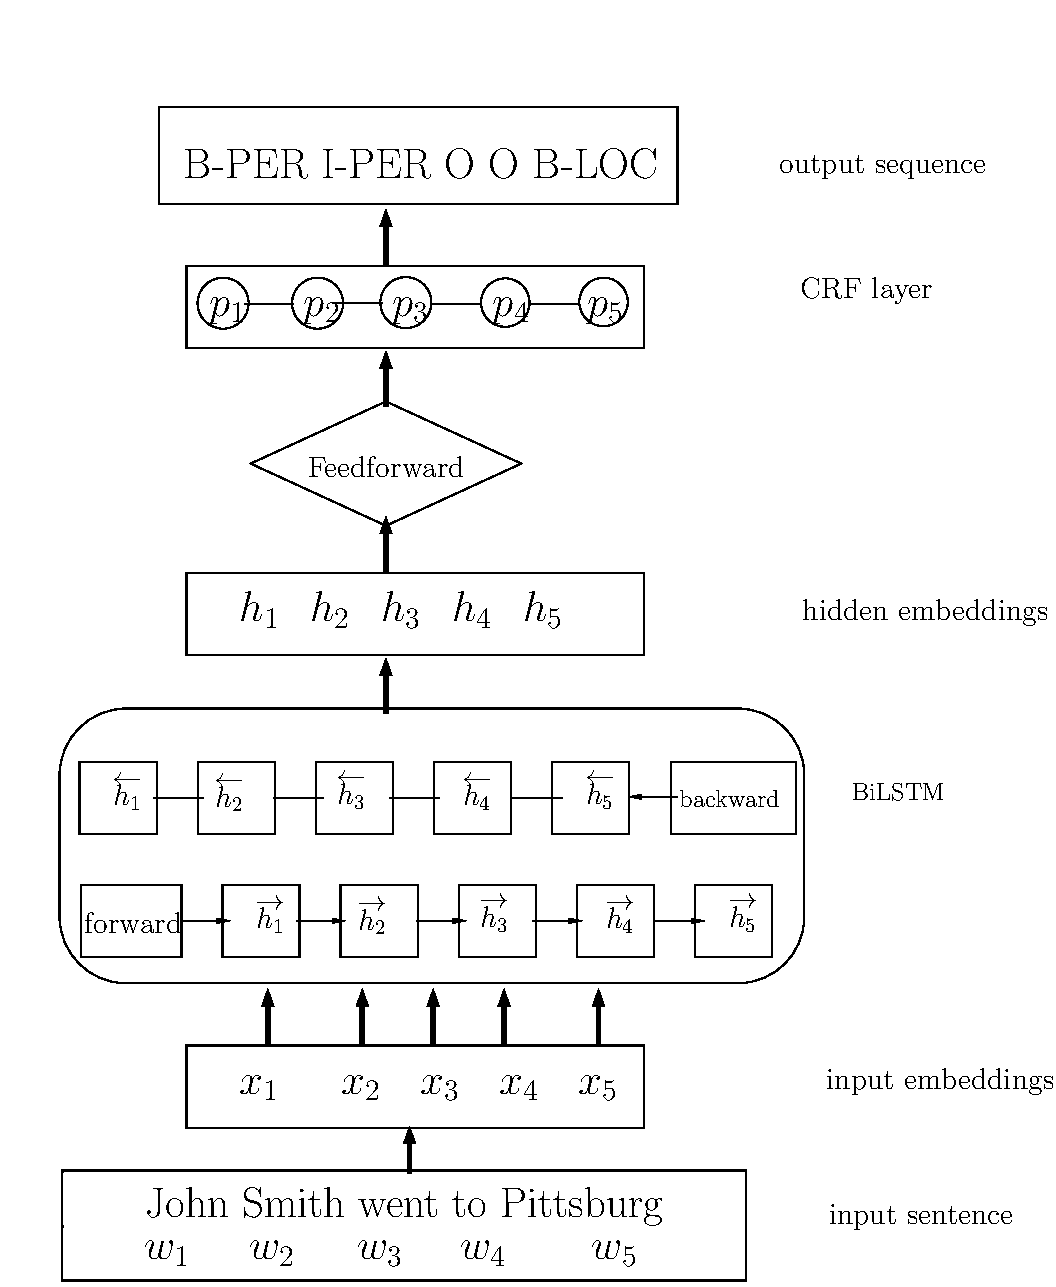
\includegraphics[scale=0.6]{bilstmcrf.pdf}
 \caption{The architecture of an NER tagging system using BiLSTM with CRF}
  \label{fig:bilstmcrf}
\end{figure}

\subsection{Character Embeddings}

Instead of using hand-engineered features listed in Chapter 2 (like prefixes and the suffixes of a word), we can use a BiLSTM network to construct word representations from characters in it (\citeauthor{lample2016neural}, \citeyear{lample2016neural}). This architecture is denoted as Character Embeddings. It has been shown that learning character embeddings has been found useful for capturing morphological evidence (\citeauthor{ling2015finding}, \citeyear{ling2015finding}). Figure \ref{fig:charlstm} describes the architecture using character embeddings and BiLSTM to generate word embedding for word "Smith". The input to the BiLSTM is the letter sequence of a word. We define a character dictionary which maps each character to a $d$-dimensional vector representation. The English character dictionary contains uppercase and lowercase letters, numbers, and punctuation. We look up each $c_{i}$ of the input letter sequence from the dictionary and get the character embedding vectors $X:\left\{x_{1},x_{2},\dots,x_{n}\right\}$. Then, character embedding vectors $X$ is fed into BiLSTM to generate forward and backward hidden embeddings of the character sequence. We concatenate the last forward hidden embedding $\overrightarrow {h_{n}}$ and the last backward hidden embedding $\overleftarrow {h_{1}}$ with the embeddings from word embedding dictionary lookup to obtain the final word embedding.

We add Character Embeddings in the sequence tagging system by concatenating the output of Character Embeddings and the word embeddings from lookup to form input embeddings. Then, we feed the input embeddings to BiLSTM and CRF, and we get the fully structured BiLSTM model (BiLSTM-Char-CRF) for sequence tagging. The character embeddings and word embeddings are learned together during training. There are existing implementations of BiLSTM-Char-CRF, such as NeuroNet by \cite{2017neuroner} which achieves state-of-the-art performance. In order to compare BiLSTM-Char-CRF with other models in this thesis, we re-implement the model.

\begin{figure}
  \centering
  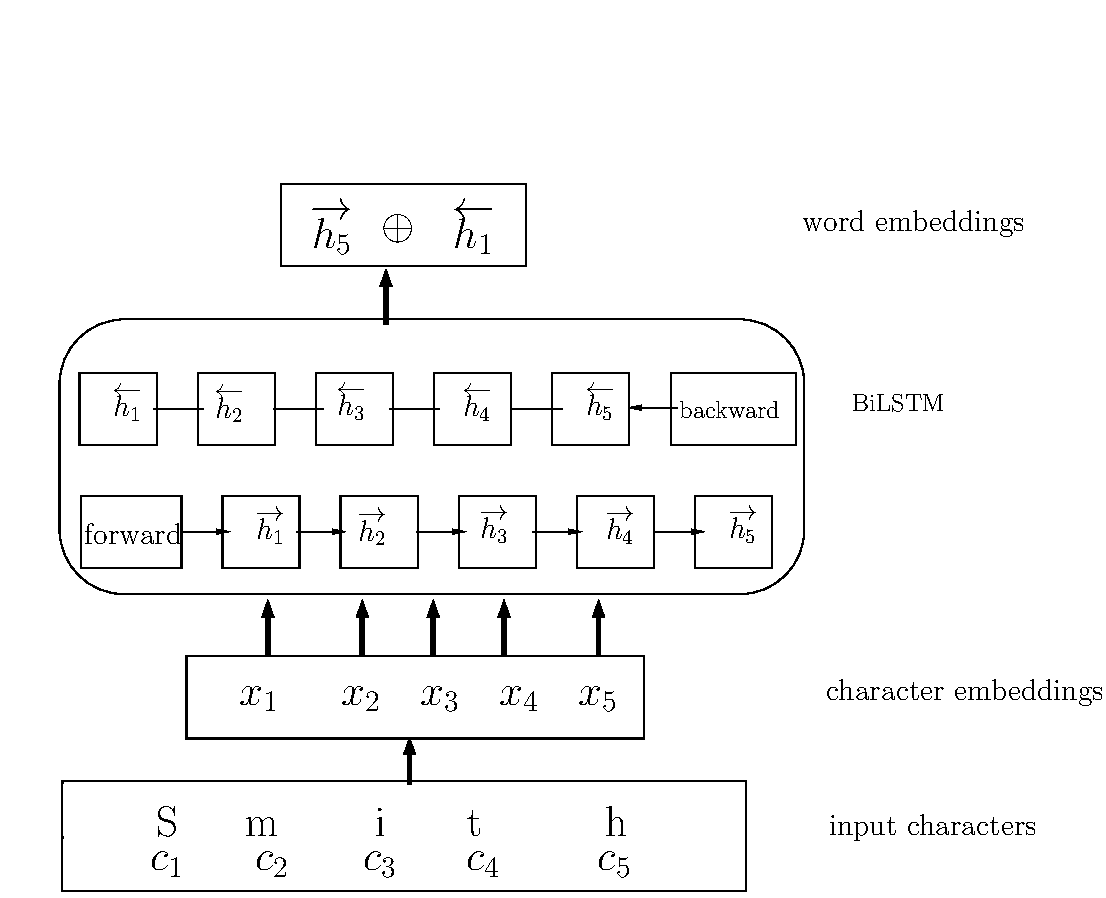
\includegraphics[scale=0.6]{bilstmchar.pdf}
 \caption{The word embedding derived from the character embeddings}
  \label{fig:charlstm}
\end{figure}


 
\section{Experiments and Results}

To evaluate BiLSTM models, we run BiLSTM with three configurations on POS and NER: BiLSTM with word features only (BiLSTM); BiLSTM with Character Embeddings (BiLSTM-Char); BiLSTM with Character Embeddings and a CRF layer (BiLSTM-Char-CRF). We report the performance and decoding speed of the models on Penn Treebank data set for POS, and on CoNLL 2003 data set for NER. 

As in the implementation for feedforward models, we implement BiLSTM models using Python and the Tensorflow 1.0 library. The hidden layer size in the BiLSTM of Character Embeddings is set to 50, and the hidden layer size in word sequence BiLSTM is set to 100. The rest of the hyperparameters are the same as the ones in the feedforward network experiments. Since dropout training (\citeauthor{hinton2012improving}, \citeyear{hinton2012improving}) can improve the performance by encouraging the model to depend on both character embeddings and word embeddings, we apply a dropout mask on the input embeddings before the BiLSTM layer. The dropout rate is set to 0.5 in the experiments. Table \ref{table:hyperparameters2} shows the hyperparameters used in BiLSTM models.

\begin{table}[]
\centering
\caption{Hyperparameters used in BiLSTM Models}
\label{table:hyperparameters2}
\begin{tabular}{|c|c|}
\hline
Hyperparameters & Values \\ \hline
character embedding size & 50 \\ \hline
word embedding size & 100 \\ \hline
feedforward layer size & 200 \\ \hline
feedforward layer & 1 \\ \hline
BiLSTM layer size & 100 \\ \hline
BiLSTM layer & 2 \\ \hline 
optimizer & Adam \\ \hline
learning rate & 0.01 \\ \hline
batch size & 32 \\ \hline
\end{tabular}
\end{table}

Figure \ref{fig:lstmbar} illustrates the performance of BiLSTM, BiLSTM-Char, and BiLSTM-Char-CRF. As expected, the fully structured BiLSTM model outperforms the other two. The structure of Character Embeddings increases POS accuracy by 1.17, and increases NER F1 score by 3.34. It reveals that the BiLSTM networks do not heavily depend on features other than words, and Character Embeddings can help improve the performance on NER more than on POS. Compared to BiLSTM-Char, BiLSTM-Char-CRF improves the POS performance by 0.13, and improves the NER performance by 1.79. CRF layer is more helpful for NER for the reason that there are grammar constraints on NER output tag sequence.

\begin{figure}
  \centering
  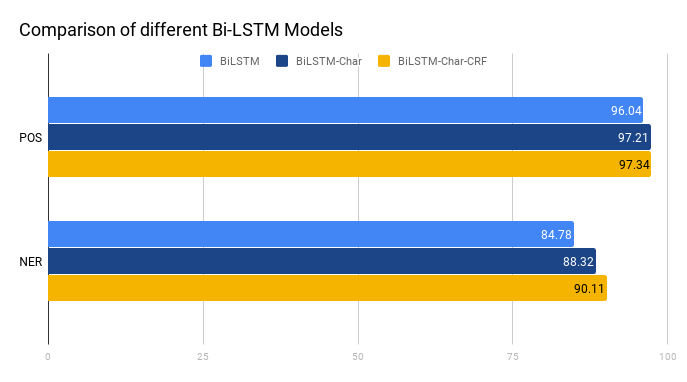
\includegraphics[scale=0.6]{lstmbar.png}
 \caption{Performance comparison between BiLSTM models on POS and NER (accuracy for POS; F1 score for NER}
  \label{fig:lstmbar}
\end{figure}


\begin{table}[]
\centering
\caption{BiLSTM Models Accuracy and F1 Score}
\label{table:lstm-table1}
\begin{tabular}{|c|c|c|}
\hline
Model         & POS (Accuracy)  & NER (F-Score)       \\ \hline
BiLSTM  & 96.01     & 84.78                             \\ \hline
BiLSTM-Char & 97.21 & 88.32             \\ \hline
BiLSTM-Char-CRF & \textbf{97.34}  & \textbf{90.11}             \\ \hline
\end{tabular}
\end{table}

\begin{table}[]
\centering
\caption{BiLSTM Models Decoding Speed}
\label{table:lstm-table2}
\begin{tabular}{|c|c|c|}
\hline
Model       & POS  (sentences, words/sec)  & NER  (sentences, words/sec)      \\ \hline
BiLSTM             & 981(23036)     & 1637(20740)       \\ \hline
BiLSTM-Char        & 596(13992)  & 889(11271)             \\ \hline
BiLSTM-Char-CRF    & 383(9009)  & 795(10100)         \\ \hline
\end{tabular}
\end{table}


Table \ref{table:lstm-table1} and Table \ref{table:lstm-table2} describe the final results of the performance and decoding speed of BiLSTM models on the POS and NER. It is obvious that the more features the model has, the slower it would be. Adding a CRF layer will increase the performance but decrease the decoding speed. 

%Table \ref{table:lstm-table3} compares the fully structured BiLSTM-Char-CRF model with Feedforward-History and Feedforward-CRF. The results reveal that considering the whole sequence in training can improve the performance, but models without recurrent structure or CRF can be faster and achieve comparable accuracy.



\iffalse
\begin{table}[]
\centering
\caption{Decoding Speed Comparison between BiLSTM Models and Feedforward Models on POS and NER}
\label{table:lstm-table3}
\begin{tabular}{|c|c|c|}
\hline
Model       & POS  (sentences, words/sec)  & NER  (sentences, words/sec)      \\ \hline
Feedforward-History            & 829(19474)     & 1390(17609)       \\ \hline
Feedforward-CRF        & 761(17877)  & 1374(17412)             \\ \hline
BiLSTM-Char-CRF    & 383(9009)  & 795(10100)         \\ \hline
\end{tabular}
\end{table}
\fi




\chapter{Feedforward Neural Network Models}

In this chapter, we describe two feedforward network models: Feedforward-History and Feedforward-CRF. Then, we show the performance and decoding speed of different feedforward models on POS and NER. 

\section{Network Architecture}

\subsection{Feedforward-History Model}

Inspired by the greedy parser system by \cite{chen2014fast}, we present a similar greedy transition system for sequence tagging in this thesis. The greedy parser system employs a basic arc-standard system (\citeauthor{nivre2004deterministic}, \citeyear{nivre2004deterministic}), which consists of three types of transitions (LEFT-ARC, RIGHT-ARC, and SHIFT), a stack, and a buffer. While the greedy parser system has three types of actions, the sequence tagging system only needs the SHIFT action which predicts the tag of the current word in the buffer and shifts the word to the stack.  Syntaxnet from Google also uses the same model for POS and dependency parsing and achieves near the state-of-the-art performance on both tasks (\citeauthor{alberti2017syntaxnet}, \citeyear{alberti2017syntaxnet}).

In our greedy tagging system, we use a feedforward network to make decisions on individual words, and we assume that the word to be labeled depends mainly on its neighbor words instead of the whole sentence. Besides the word features, the system also takes into account the lexical composition of the words (spelling features), and the previous tag decisions (previous tag features). Thereby, we represent this architecture as the Feedforward-History model. The way Feedforward-History incorporates word features is the same with the window approach proposed in \cite{collobert2011natural}. The difference between these two models is that Feedforward-History uses spelling features and previous tag features while the model in \cite{collobert2011natural} only uses word features.

\begin{figure}
  \centering
  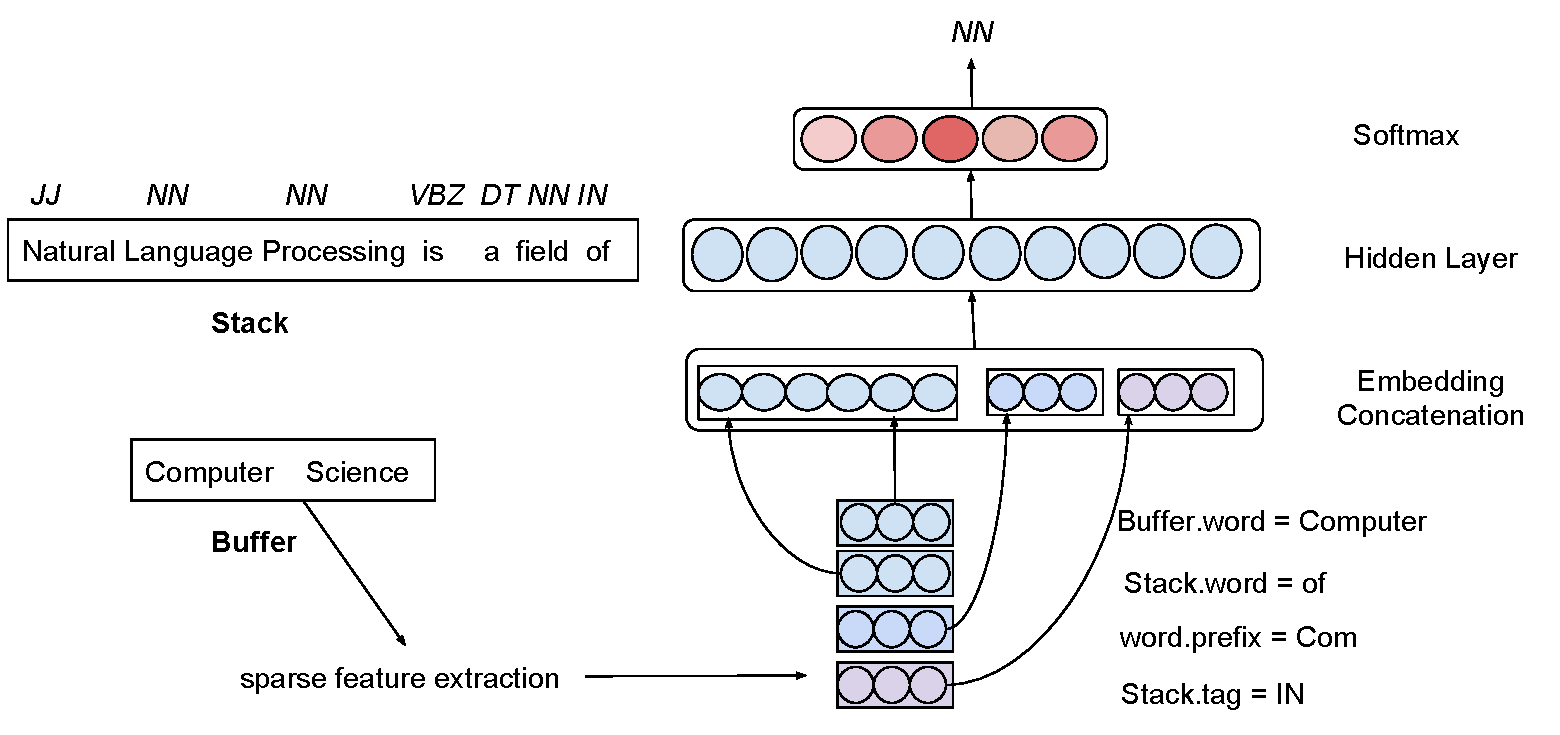
\includegraphics[scale=0.6]{greedypos.pdf}
 \caption{The architecture of a greedy tagging system using the Feedforward-History model.}
  \label{fig:greedypos}
\end{figure}

Figure \ref{fig:greedypos} illustrates the process of how a greedy tagging system uses Feedforward-History to decode a POS example. Since the focused word only depends on its neighbors in this greedy tagging system, we use a fixed size window around the current word to generate features. In order to generate features for the words at the beginning and at the end of the sentence, we add special padding words at the beginning and at the end. To generate dense word features, we convert each word in the input sequence to a $d$-dimensional vector representation $e_{w_{i}}$. Meanwhile, we have a full vocabulary embedding dictionary $E_{w}$. Given a word $w_{i}$, we look up its embedding $e_{w_{i}}$ in $E_{w}$. According to \cite{ratnaparkhi1996maximum}, spelling features of a word can help predict the part-of-speech tag. The examples of spelling features are upper and lower case features, prefix and suffix features, digit features, etc. Each spelling feature of a word is also associated with an embedding vector $e_{s_{i}}$, and it can be looked up from a embedding vector dictionary $E_{s}$. Besides word features and spelling features, we incorporate the previous tag features in this model. Each previous tag decision is represented as $e_{ht_{i}}$ and can be looked up from a tag dictionary represented as $E_{HT}$.

The input layer $X=\left( x_{1},x_{2},\ldots x_{n}\right)$ to the feedforward network is obtained by concatenating the word feature vectors, spelling feature vectors, and previous tag feature vectors. In general, generating a lot of hand-engineered features for sequence tagging is expensive: selecting useful features is an empirical process based on trials and errors, and computing feature vectors requires searching feature strings in huge dictionaries and concatenating them together. We try to use as little hand-engineered features as possible to save the time from feature generation while keeping the model accurate. In our implementation, we extract the word and spelling features on a window size of 8 centered on the focused word. We extract the following spelling features of each word: whether it starts with a capital letter; whether it has all capital letters; whether it has a mix of letters and digits; whether if has punctuation; and letter prefixes and suffices of length two and three. We also extract 4 previous tags as parts of input features.

While the input layer is the concatenation of the feature vectors of the focused word, the the output layer is a probability distribution over tags. The input unit $x_{i}$ is mapped to a hidden unit $h_{i}$ through the rectifier activation function (\textit{ReLU}) (\citeauthor{nair2010rectified}, \citeyear{nair2010rectified}):

\begin{equation}
\textit{ReLU}\left(x\right) = \textit{Max}\left(0,x\right)
\end{equation}

\begin{equation}
h_{i}=\textit{ReLU}\left( W_{1}^{w}x_{i}^{w}+W_{1}^{s}x_{i}^{s}+W_{1}^{l}x_{i}^{l}+b_{1}\right),
\end{equation}

where $x^{w}$ represents the word features, $x^{s}$ represents the spelling features, $x^{l}$ represents previous tag features, $W_{1}$ is the weight parameters in the hidden layer, and $b_{1}$ is the bias of in the hidden layer. The output of the network is a probability distribution over tags, and its dimension is the size of all tags. The tag probability distribution is modeled by a softmax layer (\textit{softmax}) (\citeauthor{dugas2001incorporating}, \citeyear{dugas2001incorporating}):

\begin{equation}
p_{i}=\textit{softmax}\left(W_{2}h_{i}+b_{2}\right),
\end{equation}

where $W_{2}$ is the weight parameter in the softmax layer and $b_{2}$ is the bias in the softmax layer. The network is trained by minimizing a negative log likelihood over the training data. Embedding vectors are trained together with weight vectors and bias in the model. We denote all trainable parameters as $\theta$. Given a sequence predictions, $Y=\left( y_{1},y_{2},\ldots y_{n}\right)$,
the score of the output sequence is the sum of the probability of each decision $y_{i}$: 

\begin{equation}
S\left( Y\right) = \sum _{i}^{n}p_{i}\left(y_{i}\right),
\end{equation}

and the loss function is:

\begin{equation}
L\left(\theta\right) = -log\left(\sum _{i}^{n}p_{i}\left(y_{i}\right)\right),
\end{equation}


\subsection{Feedforward-CRF}
\label{Feedforward-CRF}
There are two ways to incorporate output tags in the model: the first one is to use the previous predicted tags as input features to feed into the feedforward network as in Feedforward-History; the second one is to use CRF on sentence level output tags as in the following model. Feedforward-CRF shares the same architecture with Feedforward-History except using CRF to model the output sequence after computing tag probability distribution for each individual word. Feedforward-History can perform well on some sequence tagging tasks in which output labels do not have strong correlations, such as POS. Some tasks have grammar constraints on output tags so that there are strong dependencies among them, such as NER. While Feedforward-History fails to take into account the grammar constrains on the output tag sequences, Feedforward-CRF can make final decisions on the sentence level. Since the first part of the architecture is the same as Feedforward-History, we skip this part. We describe how to apply CRF to model the sequence in detail here.

Given a sequence of output predictions $y=\left( y_{1},y_{2},\ldots y_{n}\right)$,
the score of the output sequence is:

\begin{equation}
S\left( y\right)=\sum _{i}^{n}T_{i,i+1}+\sum _{i}^{n}p_{i}\left(y_{i}\right)
\end{equation}

where $T$ is a matrix of transition scores such that $T_{i,j}$ represents the score of a transition from the label $i$ to label $j$, and $p_{i}\left(y_{i}\right)$ is the probability of $y_{i}$ being the label of word $i$.

During training, we score every possible output sequence, and use a softmax layer to generate the probability distribution of output sequences, shown in Equation \ref{eqn:softmax}. Then, we minimize the negative log likelihood over the training sentences. During decoding, we can recover the tag sequences of test data using dynamic programming.

\begin{equation}\label{eqn:softmax}
P\left( y\right) = \textit{softmax}(S\left( y\right))
\end{equation}


\section{Experiments and Results}

In POS experiments, we train the models using the Penn Treebank training data and development data. Then, we decode the test data using trained models and record the per word accuracy and decoding time. In NER experiments, we train the models using the CoNLL 2003 training data and development data. Then we decode the test data using the trained models, and record the F1 score and decoding time. The details of the data sets are shown in Table \ref{table:my-dataset}. The performance of POS is measured by per word accuracy, and the performance of NER is measured by F1 score. The speed is measured by the average number of sentences and words decoded per second. We conduct experiments using \ffa{} and \ffb. We also want to show robustness of the feedforward network models, so we build a model using a feedforward network with only word features, which serves as the baseline model in our experiments. The tagging system using a feedforward network with only word features is denoted as Feedforward model in this thesis.

We implement the models using Python and the Tensorflow 1.0 library. In NER experiments, because of the small amount of training data, we use GloVE pretrained word embedding where each word corresponds to a 100-dimensional embedding vector. We use the hyper-parameters defined in the work of \cite{chen2014fast}. Specifically we use Adam (\citeauthor{kingma2014adam}, \citeyear{kingma2014adam}) for stochastic optimization, and set the learning rate to be 0.01. We use 1 hidden layer and set the hidden layer size to be 200. We have a batch implementation which can process multiple sentences at the same time, and we set the batch size to be 32 in the experiments. Table \ref{table:hyperparameters1} shows the hyperparameters. We initialize all the weight parameters using Xavier initialization (\citeauthor{glorot2011domain}, \citeyear{glorot2011domain}). To measure the speed, we run all the experiments in this thesis on a GeForce GTX 1080 GPU.

\begin{table}[]
\centering
\caption{Hyperparameters used in Feedforward Models}
\label{table:hyperparameters1}
\begin{tabular}{|c|c|}
\hline
Hyperparameters & Values \\ \hline
window size   & 8 \\ \hline
word embedding size & 100 \\ \hline
feedforward layer & 1 \\ \hline
feedforward layer size & 200 \\ \hline
optimizer & Adam \\ \hline
learning rate & 0.01 \\ \hline
batch size & 32 \\ \hline
\end{tabular}
\end{table}

\begin{table}[]
\centering
\caption{Feedforward Models Accuracy and F1 Score}
\label{table:ff-table1}
\begin{tabular}{|c|c|c|}
\hline
Model         & POS (Accuracy)  & NER (F1 Score)       \\ \hline
Feedforward    & 95.89          &   84.12     \\ \hline
Feedforward-History & 97.28     & 86.54        \\ \hline
Feedforward-CRF     & 97.30          &   87.85     \\ \hline
\end{tabular}
\end{table}

\begin{table}[]
\centering
\caption{Feedforward Models Decoding Speed}
\label{table:ff-tabel2}
\begin{tabular}{|c|c|c|}
\hline
Model       & POS  (sentences, words/sec)  & NER  (sentences, words/sec)      \\ \hline
Feedforward    & 1319(30967)     & 2117(26819)    \\ \hline
Feedforward-History & 829(19474)     & 1390(17609)     \\ \hline
Feedforward-CRF    & 761(17877)     & 1374(17412)     \\ \hline
\end{tabular}
\end{table}

\begin{figure}
  \centering
  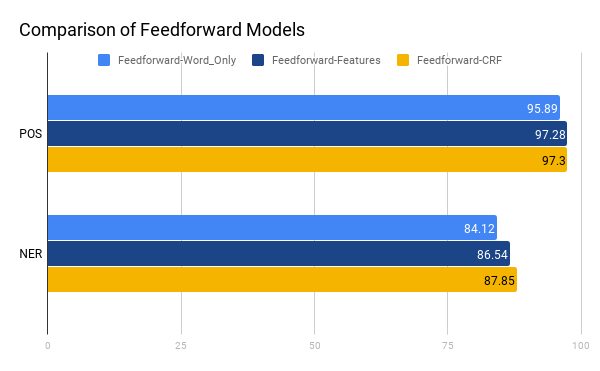
\includegraphics[scale=0.6]{ffbar.png}
 \caption{Performance comparison between Feedforward Models on POS and NER (accuracy for POS; F1 score for NER}
  \label{fig:ff}
\end{figure}


Table \ref{table:ff-table1} and Table \ref{table:ff-tabel2} present our final benchmark results of three feedforward models on POS and NER. Figure \ref{fig:ff} shows the difference in the performance of the three models. In POS, Feedforward is 1.39\% less accurate than \ffa. In NER, the F1 score of Feedforward is 2.42 lower than \ffa. Since Feedforward model with only word features does not decrease the performance dramatically, we can conclude that our greedy tagging systems with feedforward models do not heavily rely on spelling features. It also reveals that the spelling features are more helpful in NER then in POS. In both POS and NER, Feedforward-CRF has better performance than Feedforward-History, but it improves the NER performance more because of the dependencies among output tags. Feedforward-CRF is slower than Feedforward-History since CRF computes the scores of every possible output sequences.



\chapter{Mention2Vec Models}

In this chapter, we introduce multitask models based on Mention2Vec. We conduct experiments using the multitask models on sequence tagging tasks and compare their performance and decoding speed with Feedforward and BiLSTM-CRF

\section{Model Description}

\subsection{Feedforward-Mention2Vec for NER}

Mention2Vec is a neural network model for NER, which uses BiLSTMs to predict boundaries and entity types separately (\citeauthor{stratos2016mention2vec}, \citeyear{stratos2016mention2vec}). We summarize Mention2Vec into two steps. The first step uses a BiLSTM to generate hidden embeddings the same way in the BiLSTM-CRF model and predicts the boundaries using hidden embeddings. Unlike usual NER labels (B-LOC, I-LOC, \dots), boundary labels in this step do not have NER types attached. Since the boundary labels have strong correlations, Mention2Vec uses CRF to capture correlations and produce boundary label sequences.

Figure \ref{fig:mention2vec1} illustrates the first step of Mention2Vec on an NER example. We denote the input word sequence as $W: \left\{w_{1}, w_{2}, \dots, w_{n}\right\}$, input embeddings as $X: \left\{x_{1}, x_{2}, \dots, x_{n}\right\}$ which are the concatenations of the character embeddings and the word embeddings, and the hidden embeddings as $H: \left\{h_{1}, h_{2}, \dots, h_{n}\right\}$. 

\begin{figure}
  \centering
  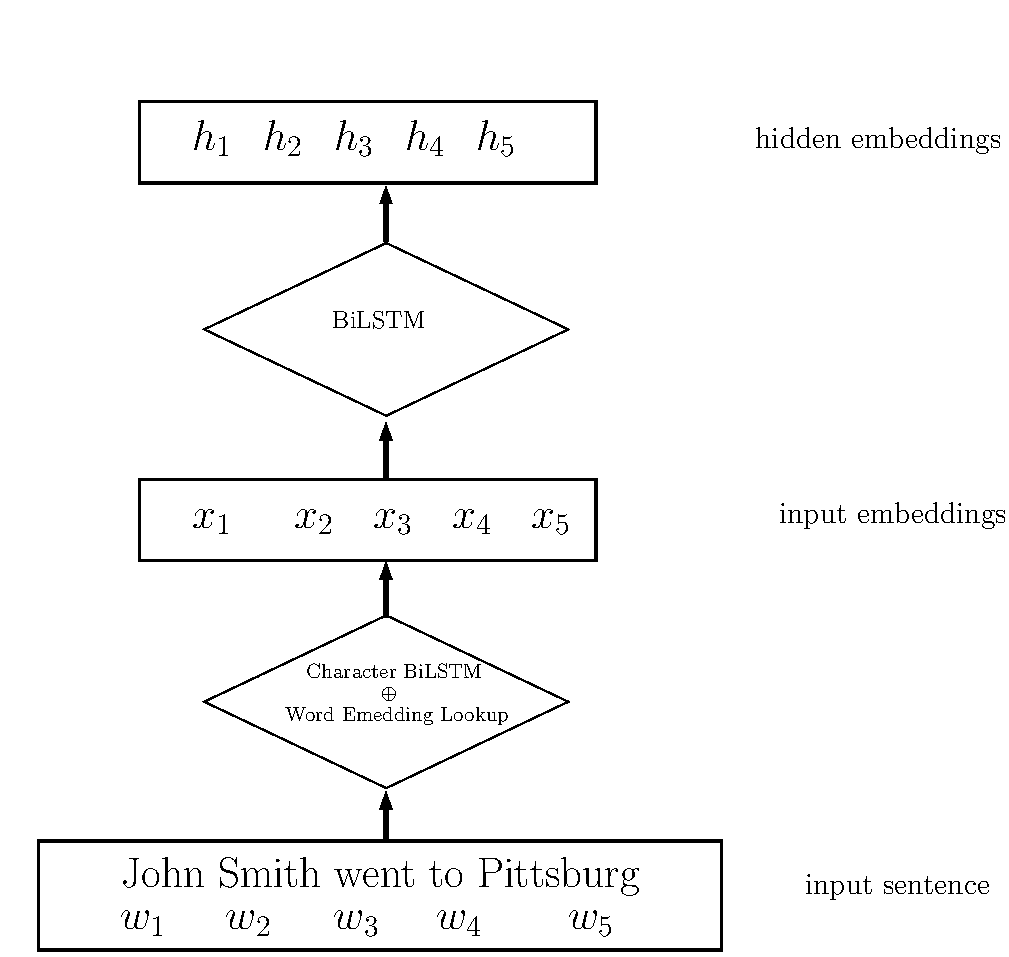
\includegraphics[scale=0.6]{mention2vec1.pdf}
 \caption{The first step of Mention2Vec for NER}
  \label{fig:mention2vec1}
\end{figure}

The output boundary label probability distribution is denoted as $p_{i}$ for word $w_{i}$, and the gold boundary label sequence is denoted as $Y_{label}$. In each training step, the boundary detection loss is given by the negative log likelihood of the gold boundary label sequence, shown in Equation \ref{eqn:loss1}

\begin{equation}\label{eqn:loss1}
  L_{1}\left(\theta _{1}\right) =-\log \left( p\left( Y_{label}|h_{1}, h_{2} \dots h_{n}\right) \right) 
\end{equation}

\begin{figure}
  \centering
  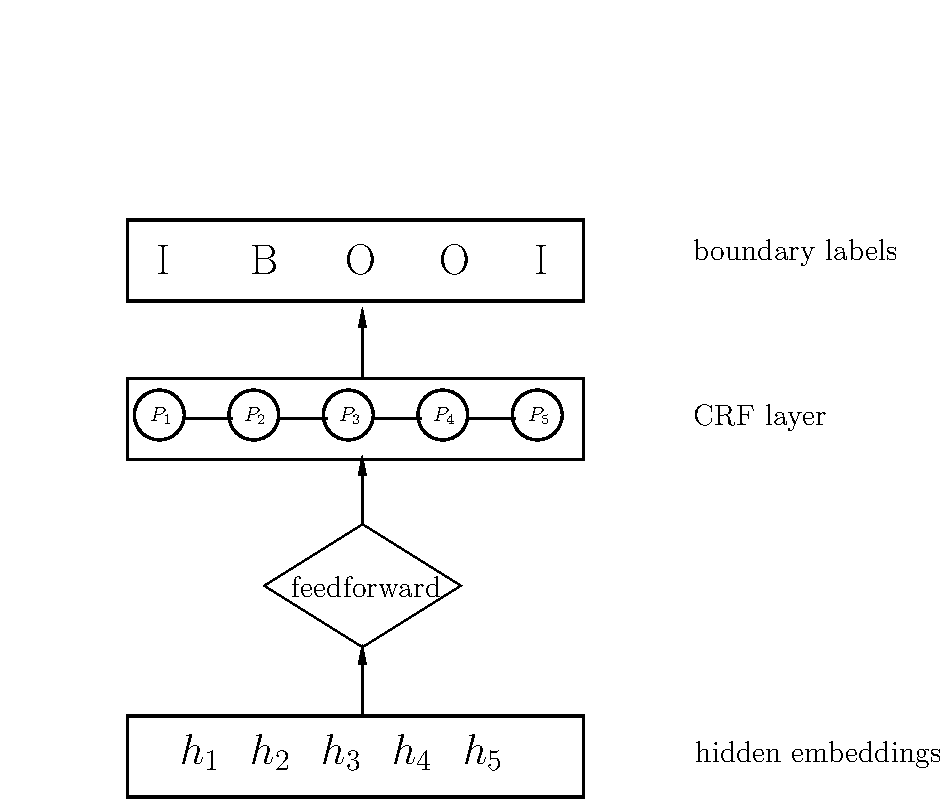
\includegraphics[scale=0.6]{mention2vec2.pdf}
 \caption{The second step of Mention2Vec for NER}
  \label{fig:mention2vec2}
\end{figure}

The second step of Mention2Vec is type prediction which finds actual types for named entity spans in a sequence. It makes use of the hidden embeddings and the entity boundaries from the first step. The model first looks up the hidden embeddings for the words in entity spans. Then, it feeds the hidden embeddings into an additional BiLSTM and obtains the type probability distributions. Figure \ref{fig:mention2vec2} illustrates the third step of Mention2Vec.

The gold type output of an input sequence is denoted as $Y_{type}$. Assuming there are $l$ named entities in a sequence, and the index of the first word in a named entity is represented as $s$, and the index of the last word in a named entity is represented as $e$, the type prediction loss is computed by \ref{eqn:loss2}:

\begin{equation}\label{eqn:loss2}
  L_{2}\left(\theta _{2}\right) =-\sum _{l}\log P\left( r^{l}|h_{s}^{l}{\ldots }h_{e}^{l}\right)
\end{equation}

During training, the model uses the gold boundaries and gold types to compute the boundary detection loss and the type prediction loss. In each training step, the boundary detection loss and the type prediction loss are minimized jointly: the training objective is to find boundary sequences and type sequences that minimize the sum of $L_{1}$ and $L_{2}$.


In order to further speed up Mention2Vec as well as capture the correlation between boundary tags, we consider using a different network for boundary detection. Shown in Chapter 3, feedforward networks can produce relatively good performance on sequence tagging with faster speed than BiLSTM. We then replace the BiLSTM in the first step of Mention2Vec with a feedforward network. We denote this new model as Feedforward-Mention2Vec. Feedforward-Mention2Vec still has two steps where the second step is the same in Mention2Vec. The first step uses a feedforward network to produce the hidden embeddings, which is illustrated in Figure \ref{fig:mention2vec3}.

\begin{figure}
  \centering
  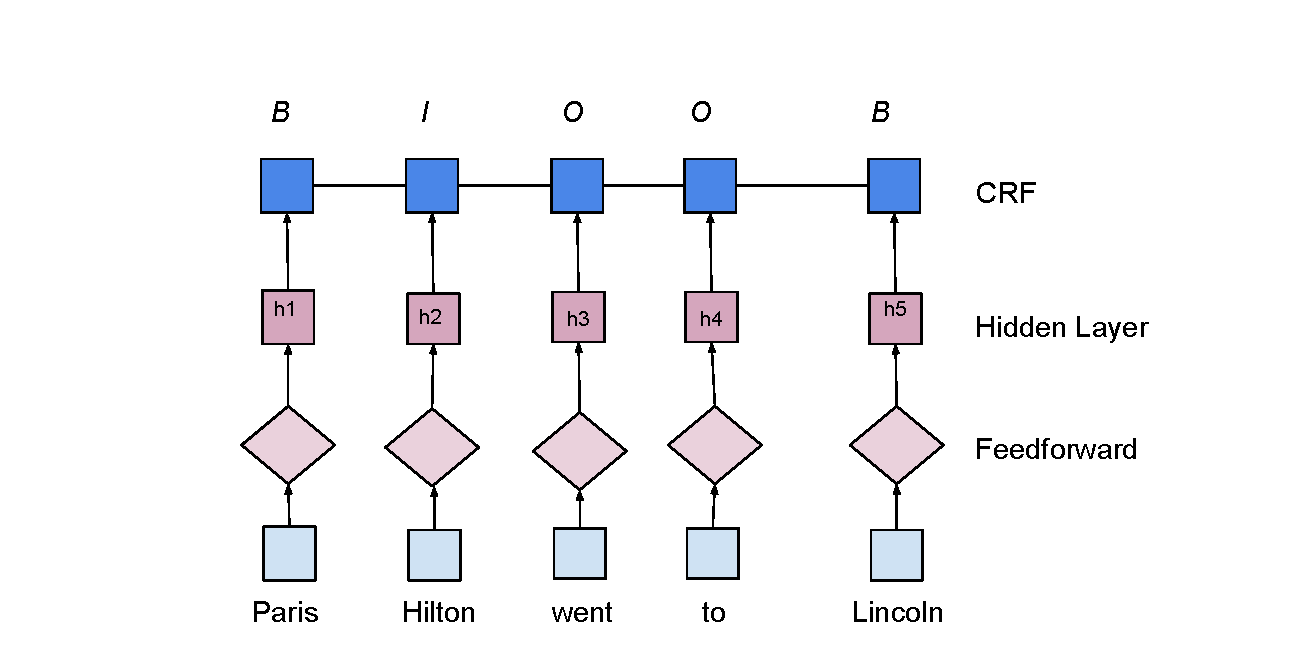
\includegraphics[scale=0.6]{mention2vec3.pdf}
 \caption{The first step of Feedforward-Mention2Vec}
  \label{fig:mention2vec3}
\end{figure}

In both Feedforward-Mention2Vec and Mention2Vec, the run time of decoding boundaries is constant with the number of types, since there are only three types of boundaries (I, O, B) to decode in the CRF layer. In other CRF based models, like BiLSTM-CRF, the decoding time grows quadratically in the number of named entity types. 

\subsection{BPE-Mention2Vec for POS}
In POS, each word in the input sentence is assigned a unique part-of-speech tag. Since there is no tag span existing in POS, it's not necessary to use a multitask model on POS. However, we propose a way to convert POS into an NER-like task through the help of Byte Pair Encoding. Inspired by the successful results obtained by using BPE in machine translation (\citeauthor{sennrich2015neural}, \citeyear{sennrich2015neural}), we initially wanted to use BPE to capture morphological decomposition of the words and replace spelling features like prefixes and suffixes. BPE is a compression algorithm which replaces frequent pairs with an unused byte. \cite{sennrich2015neural} presents a way to adapt BPE for word segmentation: using BPE to segment words into subword units of different length, and building a vocabulary dictionary using word frequency. In POS tagging system, we first learn BPE merge operations on the training data. To segment training data and test data, we first split each word in characters and then apply BPE to merge characters into larger chunks. In order to restore the words, we use the ``IOB'' label scheme to label the subword units. Since there can be multiple subword units sharing the same tag, POS becomes a task similar with NER. Figure \ref{fig:bpe} shows an example of using BPE to segment a sequence with POS tags. 

\begin{figure}[h]
  \centering
  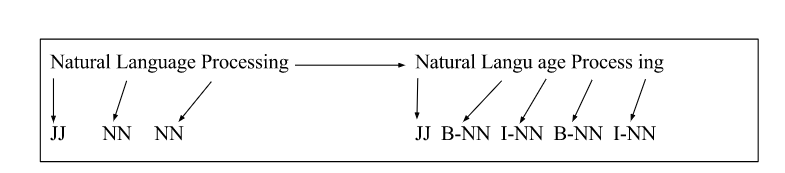
\includegraphics[scale=0.5]{bpe.png}
 \caption{An example of using BPE for word segmentation}
  \label{fig:bpe}
\end{figure}

In our proposed BPE-Mention2Vec model for POS, there are three main steps. In the first step, given a sequence, we use BPE to segment the words and convert the corresponding tags using the ``IOB'' label scheme. After the first step, we have an NER-like task with known boundary of each entity span, so we can apply the same method in Feedforward-Mention2Vec to predict the POS types for entity spans. In the second step, we use a feedforward network to produce the hidden embeddings of the input words. CRF is not used here because the boundary labels are known in both training and decoding. The third step of BPE-Mention2Vec uses a BiLSTM to predict the POS tags for each entity span based on the hidden embeddings and the known boundaries. Figure \ref{fig:bpemention2vec} describes the process of using BPE-Mention2Vec to find POS tags for a sequence. 

\begin{figure}
  \centering
  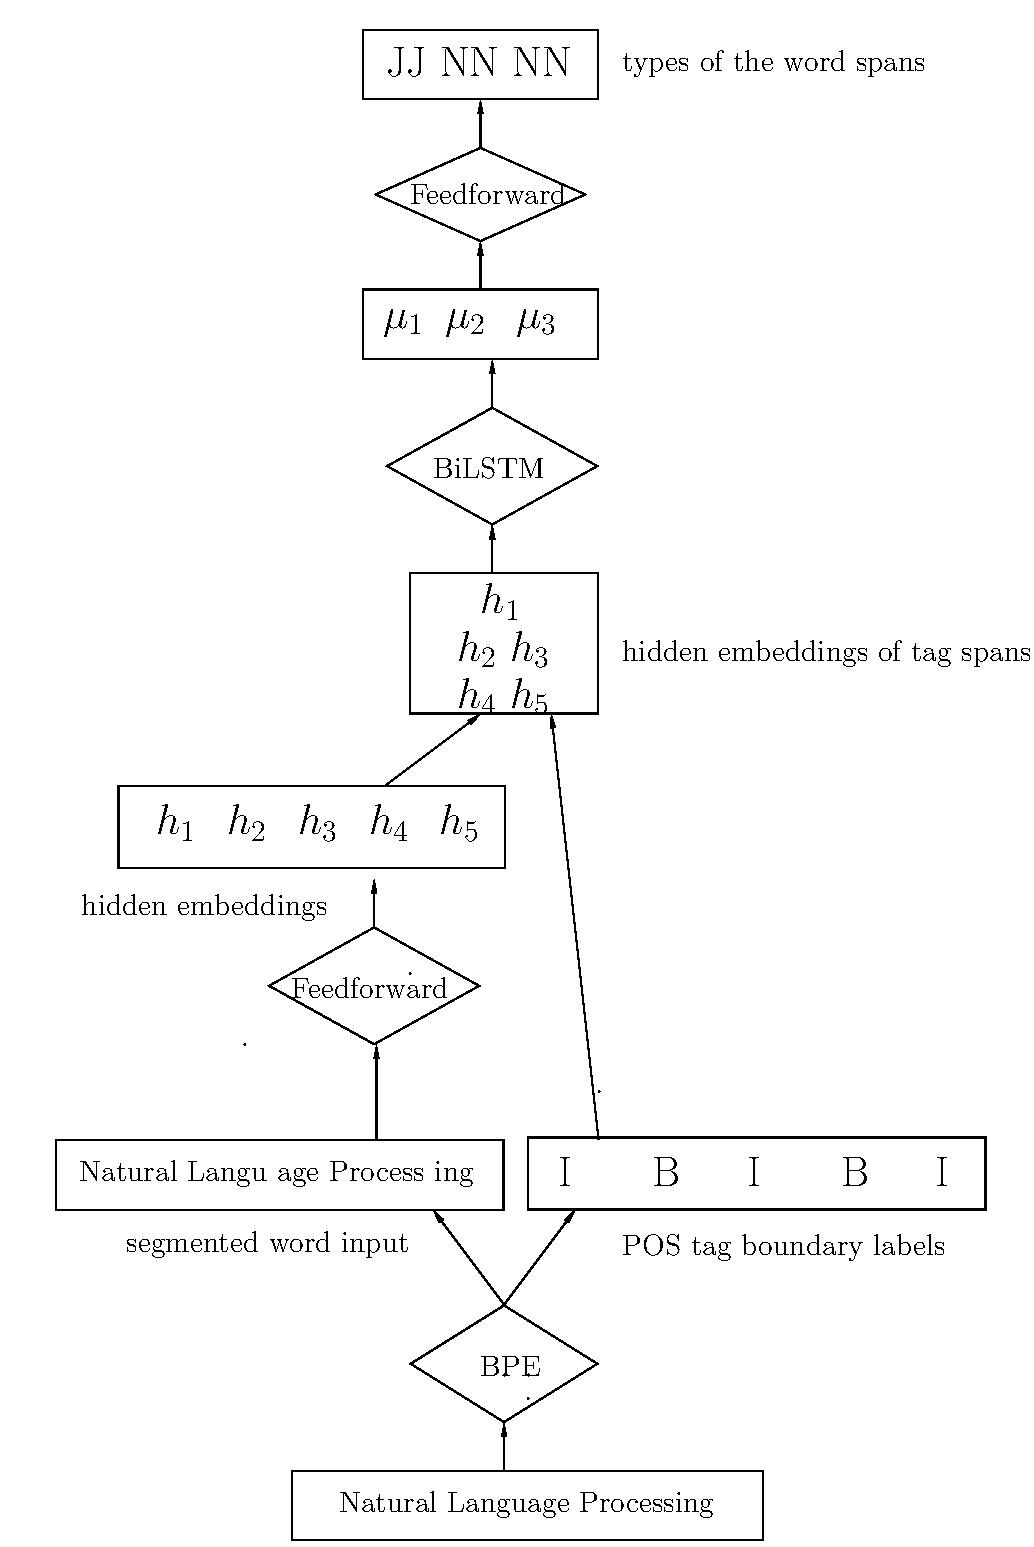
\includegraphics[scale=0.6]{bpemention2vec.pdf}
 \caption{An example of using BPE-Mention2Vec to find POS tags}
  \label{fig:bpemention2vec}
\end{figure}

\section{Experiments and Results}

We empirically evaluate the Mention2Vec model and the Feedforward-Mention2Vec model for NER, and the BPE-Mention2Vec model for POS. The hardware specifications are listed in Table \ref{table:hardware}. The experiments were conducted on a Linux server with a single 10G Nvidia GeForce GPU. The experiments specification is shown in Table \ref{table:hardware}. In the implementation of Mention2Vec, we use the same set of hyperparameters from the origin model (\citeauthor{stratos2016mention2vec}, \citeyear{stratos2016mention2vec}). We perform minimum hyperparameter tuning for Feedforward-Mention2Vec and BPE-Mention2Vec over hidden layer size, learning rate, and dropout rate. The hyperparameters we use in Feedforward-Mention2Vec and BPE-Mention2Vec are shown in Table \ref{table:hyperparameters3}.

\begin{table}[h]
\centering
\caption{Hyperparameters used in Feedforward-Mention2Vec and BPE-Mention2Vec}
\label{table:hyperparameters3}
\begin{tabular}{|c|c|}
\hline
Hyperparameters & Values \\ \hline
character embedding size & 50 \\ \hline
word embedding size & 100 \\ \hline
feedforward layer size & 200 \\ \hline
feedforward layer & 1 \\ \hline
optimizer & Adam \\ \hline
learning rate & 0.001 \\ \hline
batch size & 32 \\ \hline
dropout rate & 0.5 \\ \hline
\end{tabular}
\end{table}

\begin{table}[h]
\centering
\caption{NER F1 Score and Decoding Speed Comparison on CoNLL 2003}
\label{table:ner-mention2vec1}
\begin{tabular}{|c|c|c|c|c|}
\hline
Model   & Precision & Recall & F1 & Speed \\ \hline
Feedforward &82.99 &83.59 &83.29 & 26819 \\ \hline
BiLSTM-CRF &89.93 &90.16 &\textbf{90.05} (+6.76) & 10100 (-2.65$\times$) \\ \hline
Mention2Vec &89.14 &88.99 &89.06 (+5.77) & 9701 (-2.76$\times$) \\ \hline
Feedforward-Mention2Vec &88.98 &88.21 &88.6 (+5.31) & 13450 (-1.99$\times$) \\ \hline
\end{tabular}
\bigskip
\caption{Chunking F1 Score and Decoding Speed Comparison on CoNLL 2000}
\label{table:chunk-mention2vec1}
\begin{tabular}{|c|c|c|c|c|}
\hline
Model   & Precision & Recall & F1 & Speed \\ \hline
Feedforward & 89.35 &91.55 &90.43 & 16920 \\ \hline
BiLSTM-CRF &93.91 &93.81 &\textbf{93.86} (+3.43) & 5390 (-3.14$\times$) \\ \hline
Mention2Vec &93.03 & 93.13 &93.08 (+2.65) & 5465 (-3.09$\times$) \\ \hline
Feedforward-Mention2Vec &92.61 & 92.62 &92.61 (+2.18) & 7601 (-2.23$\times$) \\ \hline
\end{tabular}
\end{table}

\begin{table}[h]
\centering
\caption{NER F1 Score and Decoding Speed Comparison on OntoNotes}
\label{table:ner-mention2vec2}
\begin{tabular}{|c|c|c|c|c|}
\hline
Model & Precision & Recall & F1 & Speed(words/sec) \\ \hline
Feedforward  & 82.98 & 62.09 & 71.03 & 22829 \\ \hline
BiLSTM-CRF &86.59 &85.21 &\textbf{85.90} & 7667 (-2.97$\times$)
  \\ \hline
Mention2Vec & 86.24 & 84.25 & 85.23 & 8433 (-2.71$\times$)
         \\ \hline
Feedforward-Mention2Vec & 85.40 & 79.92 & 82.57 & 10812 (-2.11$\times$) \\ \hline
\end{tabular}
\bigskip
\caption{Per-label F1 Score on OntoNotes}
\label{table:ner-mention2vec3}
\begin{tabular}{|c|c|c|c|}
\hline
Labels             & Feedforward & Feedforward-Mention2Vec & BiLSTM-Char-CRF \\ \hline
         CARDINAL  & 72.38  & 78.03  & 80.33 \\ \hline
             DATE: & 72.45  & 80.61  & 81.24 \\ \hline
            EVENT: & 30.01  & 45.81  & 61.40 \\ \hline
              FAC: & 29.08  & 46.27  & 57.94 \\ \hline
              GPE: & 89.62  & 92.84  & 94.84 \\ \hline
         LANGUAGE: & 45.16  & 43.42  & 51.43 \\ \hline
              LAW: & 20.02  & 43.62  & 57.97 \\ \hline
              LOC: & 52.79  & 64.71  & 73.51 \\ \hline
            MONEY: & 77.73  & 81.66  & 86.98 \\ \hline
             NORP: & 84.11  & 87.80  & 92.15 \\ \hline
          ORDINAL: & 71.26  & 72.77  & 77.24 \\ \hline
              ORG: & 72.05  & 79.92  & 85.27 \\ \hline
          PERCENT: & 84.43  & 89.27  & 88.73 \\ \hline
           PERSON: & 82.72  & 86.98  & 90.65 \\ \hline
          PRODUCT: & 51.66  & 50.00  & 64.38 \\ \hline
         QUANTITY: & 65.78  & 74.77  & 81.13 \\ \hline
             TIME: & 41.68  & 56.44  & 58.85 \\ \hline
      WORK OF ART: & 26.29  & 37.63  & 47.21 \\ \hline
\end{tabular}
\end{table}


In Chunking and NER experiments, we compare Feedforward-Mention2Vec with Mention2Vec on the CoNLL 2003 data set. We use the BiLSTM-CRF and Feedforward as baseline models because BiLSTM-CRF achieves the highest F1 score and Feedforward has the fastest decoding speed among the previous models we built. Table \ref{table:ner-mention2vec1} shows the NER performance and decoding speed of these neural network models on the CoNLL 2003 data set.Table \ref{table:chunk-mention2vec1} shows the Chunking performance and decoding speed of these neural network models on the CoNLL 2000 data set. Mention2Vec and Feedforward-Mention2Vec obtain lower F1 score than BiLSTM-CRF. Feedforward-Mention2Vec is faster than Mention2Vec and BiLSTM-CRF. The empirical results demonstrate that the Feedforward-Mention2Vec model performs competitively on Chunking and NER while being faster than original Mention2Vec model and the state-of-the-art model. Feedforward is still the fastest but it has the lowest F1 score on both tasks.

Different NER corpus may have different named entity types. We have noted that Feedforward-Mention2Vec and Mention2Vec scale linearly in the number of named entity types while BiLSTM-CRF grows quadratically. We want to show the time difference of the same model on NER data sets with different numbers of named entity types. We have obtained the performance and decoding speed of these models on CoNLL 2003 which has 4 types of named entity. Then we conduct the experiments on the OntoNotes English data set which has 18 types of named entity. Table \ref{table:ner-mention2vec2} reports the final results of the experiments. The same model obtains lower F1 score on OntoNotes. Table \ref{table:ner-mention2vec3} shows the per label performance of Feedforward-Mention2Vec, BiLSTM-CRF, and Feedforward. They reveal that some labels in OntoNotes are classified poorly, such as ``WORK OF ART'' and ``LANGUAGE''. We suspect this is due to OntoNotes is more noisy than CoNLL 2003 as OntoNotes data is extracted from a wide variety of sources with more named entity types. In terms of decoding speed, while Feedforward-Mention2Vec is 1.3 times faster than the BiLSTM-CRF model on the data set with 4 named entity types, Feedforward-Mention2Vec is 1.4 times faster on the data set with 18 named entity types. Mention2Vec is slightly slower than BiLSTM--CRF on CoNLL 2003, but it's faster than BiLSTM-CRF on OntoNotes.

\begin{table}[h]
\centering
\caption{POS Tagging Systems Performance and speed Comparison}
\label{table:pos-mention2vec}
\begin{tabular}{|c|c|c|c|}
\hline
Model   & Accuracy & Error Reduction & Speed \\ \hline
Feedforward     & 95.89  & $-$ & 30967  \\ \hline
BPE-Mention2Vec & 96.04 (+0.15) &85 & 4923 (-6.29$\times$)   \\ \hline
BILSTM-CRF & 97.34 (+1.45) &822 & 9009 (-3.43$\times$) \\ \hline
\end{tabular}
\end{table}

In the POS experiments, we compare BPE-Mention2Vec with BiLSTM-CRF which is the state-of-the-art model for POS, and with Feedforward which is the fastest among the models we have built. Table \ref{table:pos-mention2vec} demonstrates the performance and decoding speed of them on the Penn Treebank data set. BPE-Mention2Vec obtains lower accuracy than BiLSTM-CRF and higher accuracy than Feedforward. Since using word segmentation increases the number of words to be processed and introduces more preprocessing time, BPE-Mention2Vec is slower than the BiLSTM-CRF and Feedforward. The empirical results conclude that BiLSTM-CRF is a better model than BPE-Mention2Vec on POS. 


\chapter{Discussion}

In this Chapter, we put together the final experiment results of the network models presented in this thesis, and provide an analysis of the results.

Table \ref{table:my-label1} records the performance of the neural network models for POS, NER, and Chunking. The POS performance is measured on the Penn Treebank test data set, the NER performance is measured on the CoNLL 2003 test data set, and the Chunking performance is measured on CoNLL 2000 test data set. Table \ref{table:my-label1} also includes the results from the state-of-the-art models. While our implementations obtain lower accuracy scores and F1 scores than the state-of-art results, we emphasize that our main goal of this thesis is to compare different neural networks. Since the performance scores of the state-of-the-art model are already high, we are willing to trade in some performance scores for speed improvement. Figure \ref{fig:comp1} and Figure \ref{fig:comp2} display two NER examples extracted from CoNLL 2003 test data where BiLSTM-CRF performs better than Feedforward-History and Feedforward-Mention2Vec. 


\begin{table}[h]
\centering
\caption{Neural Network Models Accuracy and F1 Score}
\label{table:my-label1}
\begin{tabular}{|c|c|c|c|}
\hline
Model        & Penn Treebank & CoNLL 2003 & CoNLL 2000     \\ \hline
\text{\cite{ling2015finding}} & \textbf{97.78} & $-$ & $-$ \\ \hline
\text{\cite{lample2016neural}} & $-$ & \textbf{90.94}  & $-$\\ \hline 
\makecell{\text{\cite{shen2005voting}} \\ \text{\cite{gut-besser-chunker}}} & $-$  & $-$ & \makecell{\textbf{95.23} \\ 95.08}\\ \hline 
Feedforward    & 95.89          & 83.29   & 90.43  \\ \hline
Feedforward-History & 97.28     & 87.47   & 92.61     \\ \hline
BiLSTM  & 96.1    & 83.74     & 91.79         \\ \hline
BiLSTM-Char & 97.21 & 87.93     & 92.98       \\ \hline
BiLSTM-CRF & \textit{97.34}  & \textit{90.05}  & \textit{93.86}     \\ \hline
Mention2Vec  & $-$    & 89.06  & 93.08  \\ \hline
Feedforward-Mention2Vec  & $-$    & 88.6  & 92.61  \\ \hline
BPE-Mention2Vec & 96.04  & $-$   & $-$   \\ \hline   
\end{tabular}
\end{table}


\begin{figure}
\begin{subfigure}{\linewidth}
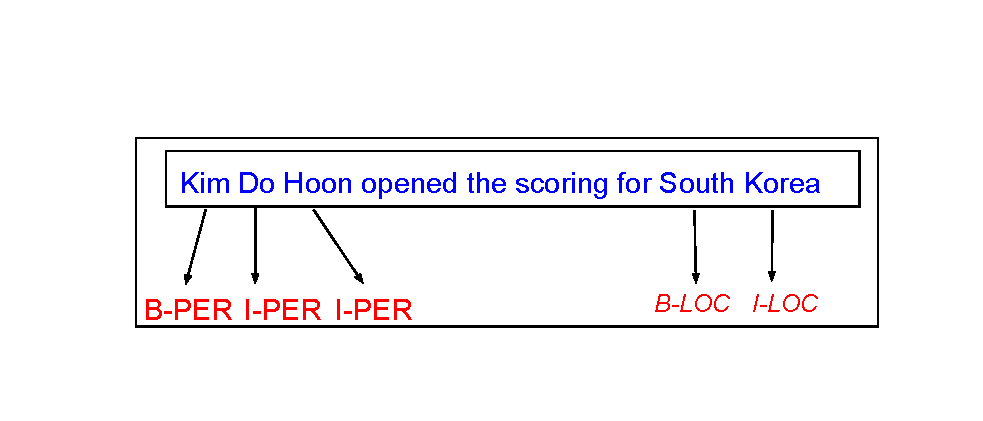
\includegraphics[width=0.9\linewidth]{NERbilstm.pdf}
\vspace{-1cm}
\caption{Result Obtained by BiLSTM-CRF}
\end{subfigure}\par\medskip
\begin{subfigure}{\linewidth}
\vspace{-2cm}
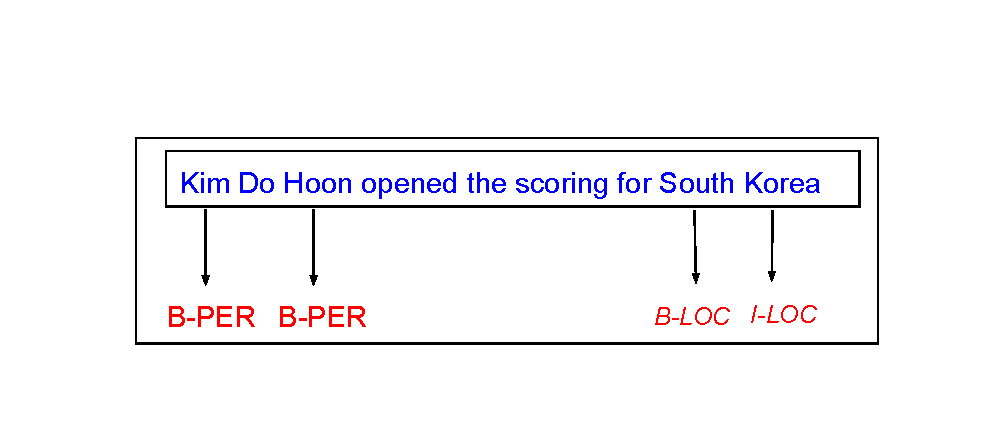
\includegraphics[width=0.9\linewidth]{NERff.pdf}
\vspace{-1cm}
\caption{Result Obtained by Feedforward-History}
\end{subfigure}
\caption{An Comparison between BiLSTM-CRF and Feedforward-History on an NER Example}
\label{fig:comp1}
\end{figure}

\begin{figure}
\centering
\begin{subfigure}{\linewidth}
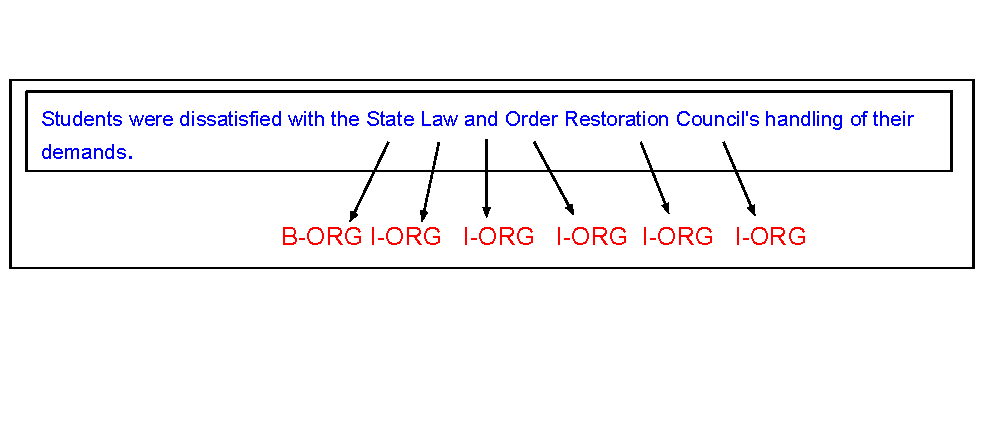
\includegraphics[width=1.0\linewidth]{NERbilstm2.pdf}
\vspace{-2.5cm}
\caption{Result Obtained by BiLSTM-CRF}
\end{subfigure}\par\medskip
\begin{subfigure}{\linewidth}
\vspace{-1cm}
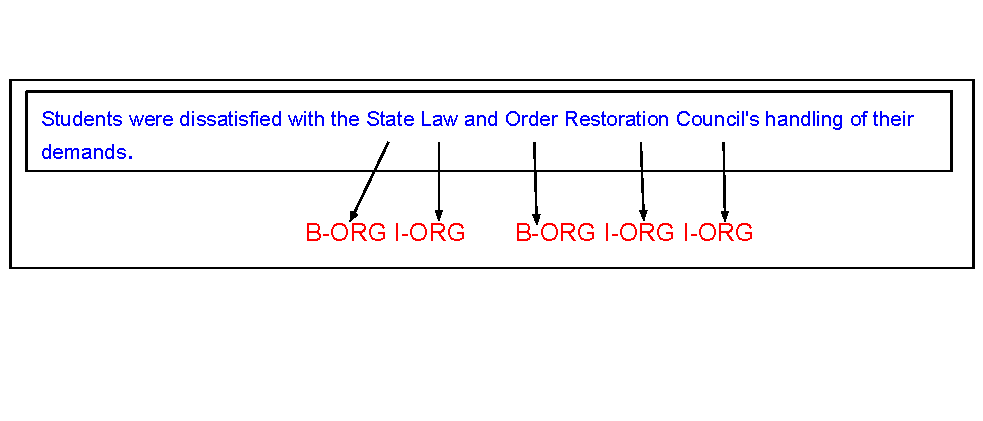
\includegraphics[width=1.0\linewidth]{NERmen.pdf}
\vspace{-2.5cm}
\caption{Result Obtained by Feedforward-Mention2Vec}
\end{subfigure}
\caption{An Comparison between BiLSTM-CRF and Feedforward-Mention2Vec on an NER Example}
\label{fig:comp2}
\end{figure}


\begin{table}[h]
\centering
\caption{Neural Network Models Decoding Speed}
\label{table:my-label2}
\begin{tabular}{|c|c|c|c|}
\hline
Model & Penn Treebank & CoNLL 2003 & CoNLL 2000\\ \hline
Feedforward    & 30967    & 26819   & 16920 \\ \hline
BiLSTM              & 23036    & 20740  & 10321    \\ \hline
Feedforward-History & 19474    & 17609  & 10067   \\
\hline
Feedforward-Mention2Vec     & $-$      & 13450 & 7601 \\ \hline
BiLSTM-Char         & 13992    & 11271  & 6616         \\ \hline
BiLSTM-CRF     & 9009     & 10100  & 5390     \\ \hline
BPE-Mention2Vec     & 4923  &  $-$  & $-$       \\ \hline   
\end{tabular}
\end{table}

Table \ref{table:my-label2} records the decoding speed of different neural network models on the Penn Treebank, CoNLL 2003 and CoNLL 2000 test data. The models are sorted by their decoding speed in descending order. The decoding speed is measured by the number of words decoded per second in the test time. It is obvious that the fewer features used in the same model the faster the decoding speed of the model will be. In general, the greedy tagging systems using feedforward models are faster then the systems using BiLSTM models. Since the CRF based models introduce a transition matrix and uses dynamic programming algorithm to decode the sequence, they are slower than the models without the CRF layer.


\begin{figure}[h]
\centering
  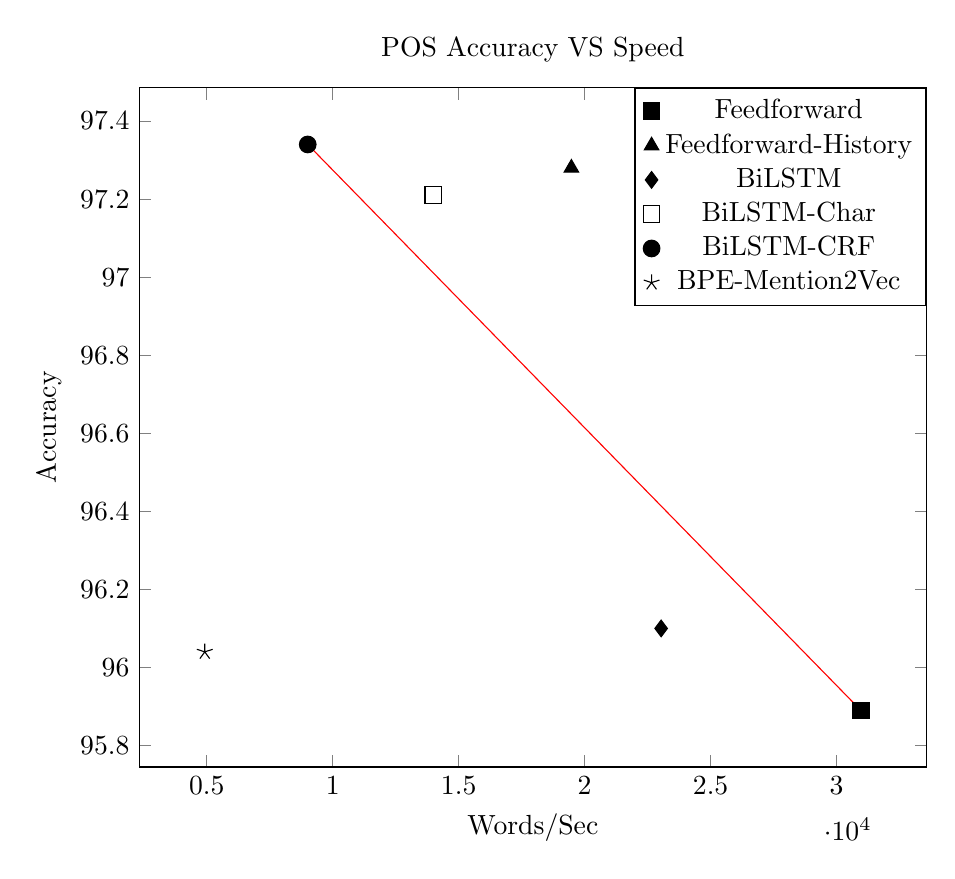
\begin{tikzpicture}
	\begin{axis}[%
	ylabel={Accuracy},
	xlabel={Words/Sec},
	scale only axis,
	mark size=3.0pt,
	title={POS Accuracy VS Speed},
	scatter/classes={%
		Feedforward={mark=square*},%
		Feedforward-History={mark=triangle*},%
		BiLSTM={mark=diamond*},%
		BiLSTM-Char={mark=square},
		BiLSTM-CRF={mark=otimes*},%
		BPE-Mention2Vec={mark=star}},%
	legend style={at={(1,1)},anchor=north east,
    draw=black,fill=white,align=left}]
	\addplot[scatter,only marks,%
		scatter src=explicit symbolic]%
	table[meta=label] {
    x     y      label
    30967  95.89  Feedforward 
    19474  97.28  Feedforward-History 
    23036  96.1   BiLSTM
    13992  97.21  BiLSTM-Char
    9009   97.34  BiLSTM-CRF
    4923   96.04  BPE-Mention2Vec
    };
    \addplot+ [mark=none]table {
    x     y      label
    30967   95.89   Feedforward  
    9009   97.34    BiLSTM-CRF
    };
	\addlegendentry{Feedforward}
	\addlegendentry{Feedforward-History}
	\addlegendentry{BiLSTM}
	\addlegendentry{BiLSTM-Char}
	\addlegendentry{BiLSTM-CRF}
	\addlegendentry{BPE-Mention2Vec}
	\end{axis}
\end{tikzpicture}
 \caption{Results of the POS system using different Neural Network Models}
  \label{fig:pos}
\end{figure}

Figure \ref{fig:pos} illustrates the trade-off between performance and decoding speed in POS systems using different neural network models. Among the neural network models for POS, BiLSTM-CRF achieves the best per word accuracy 97.34\%, and Feedforward-History obtains the second best per word accuracy 97.28\%. Feedforward achieves the fastest decoding speed since it employs a simple neural network without extra features. The line in Figure \ref{fig:pos} connects BiLSTM-CRF which is the most accurate model and Feedforward which is the fastest model. The models above the line are faster but perform slightly worse than BiLSTM-CRF, such as Feedforward-History and BiLSTM-Char. Models below the line such as BPE-Mention2Vec are slower and less accurate, which makes them less ideal for POS. Feedforward-History is the fastest model with competitive performance on POS, and it is about 2 times faster than BiLSTM-CRF.

\begin{figure}[h]
\centering
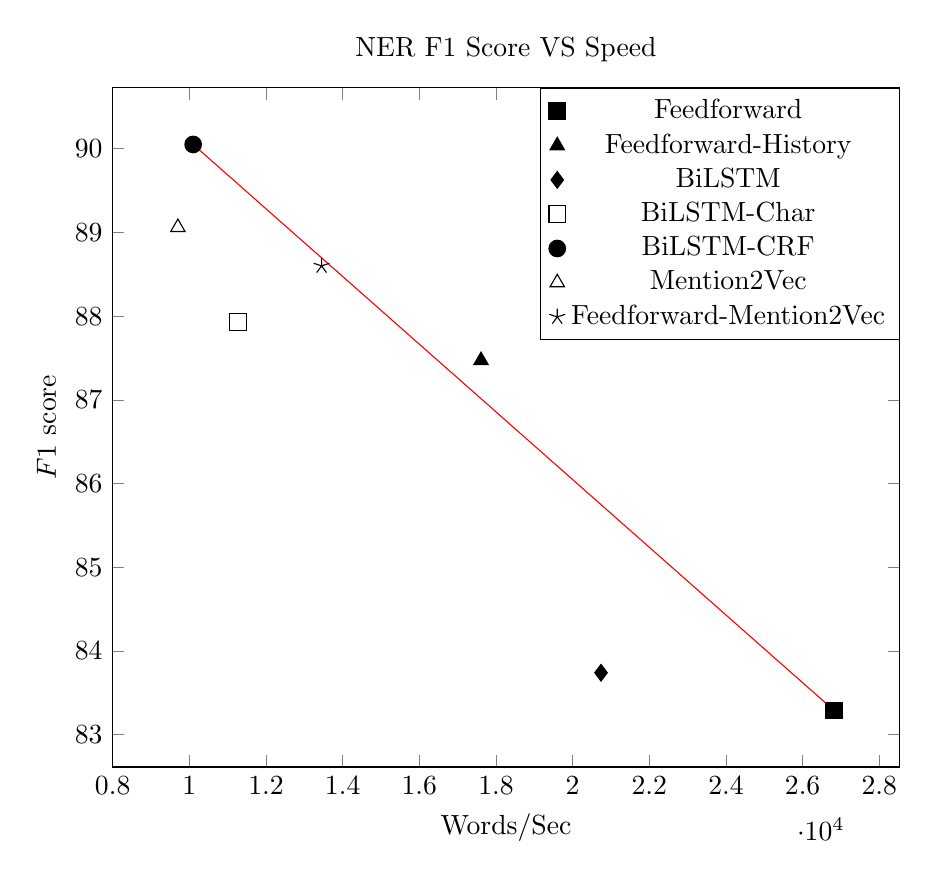
\begin{tikzpicture}
	\begin{axis}[%
	ylabel={$F1$ score},
	xlabel={Words/Sec},
	scale only axis,
	mark size=3.0pt,
	title={NER F1 Score VS Speed},
	scatter/classes={%
		Feedforward={mark=square*},%
		Feedforward-History={mark=triangle*},%
		BiLSTM={mark=diamond*},%
		BiLSTM-Char={mark=square},
		BiLSTM-CRF={mark=otimes*},%
		Mention2Vec={mark=triangle},
		Feedforward-Mention2Vec={mark=star}},%
	legend style={at={(1,1)},anchor=north east,
    draw=black,fill=white,align=left}]
	\addplot[scatter,only marks,%
		scatter src=explicit symbolic]%
	table[meta=label] {
    x     y      label
    26819   83.29   Feedforward 
    17609   87.47   Feedforward-History 
    20740   83.74   BiLSTM 
    11271   87.93   BiLSTM-Char
    10100   90.05   BiLSTM-CRF
    9701    89.06   Mention2Vec
    13450   88.6   Feedforward-Mention2Vec
	};
	\addplot+ [mark=none]table {
    x     y      label
    26819   83.29    Feedforward 
    10100   90.05   BiLSTM-CRF
    };
	\addlegendentry{Feedforward}
	\addlegendentry{Feedforward-History}
	\addlegendentry{BiLSTM}
	\addlegendentry{BiLSTM-Char}
	\addlegendentry{BiLSTM-CRF}
	\addlegendentry{Mention2Vec}
	\addlegendentry{Feedforward-Mention2Vec}
	\end{axis}
\end{tikzpicture}
 \caption{Results of the NER system using different Neural Network Models on CoNLL 2003}
  \label{fig:ner}
\end{figure}

Figure \ref{fig:ner} illustrates the trade-off between performance and speed of using different neural network models on CoNLL 2003. BiLSTM--CRF achieves the highest F1 Score 90.05, and Mention2Vec obtains the second best F1 Score 89.06. Feedforward achieves the fastest decoding speed since it employs a simple neural network with no extra features. The line in Figure \ref{fig:ner} connects the BiLSTM-CRF model which is the most accurate model and the Feedforward model which is the fastest model. The models above the line are faster but perform slightly worse than BiLSTM-CRF, such as Feedforward-History. Our new model, Feedforward-Mention2Vec, comes very close to the line, and it achieves 88.6 F1 score which is close to the best performance, and it is 1.3 times faster than the fully structured BiLSTM model.


\begin{figure}[h]
\centering
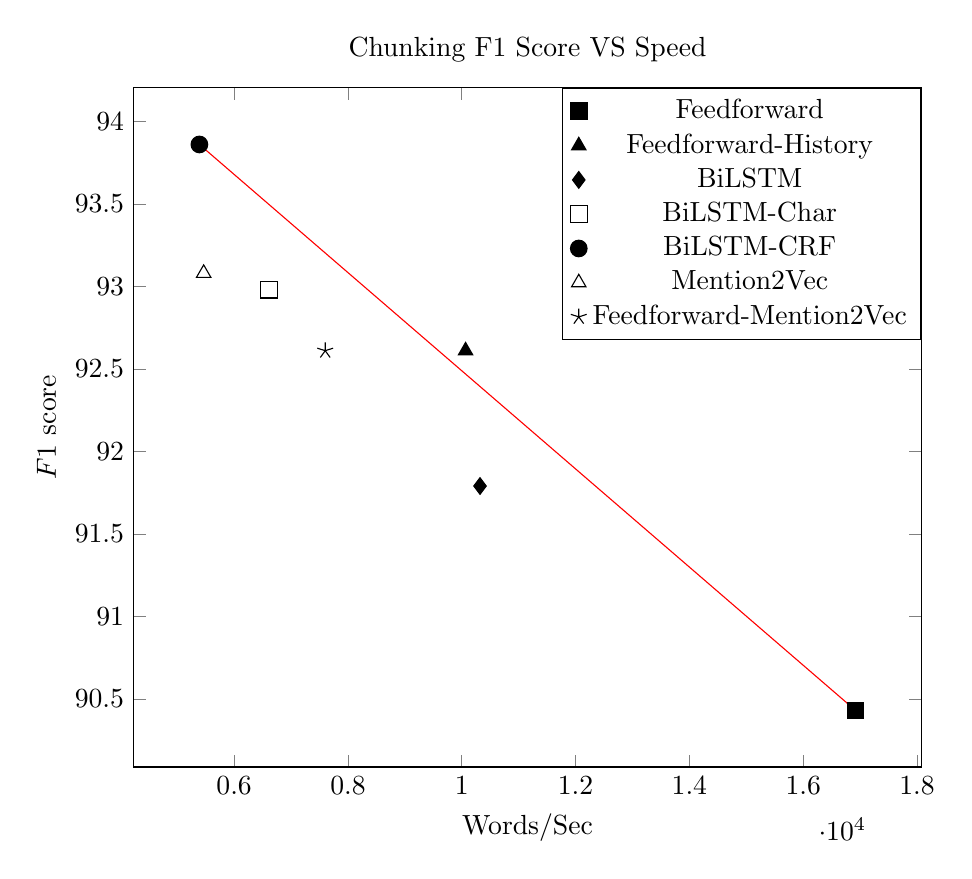
\begin{tikzpicture}
	\begin{axis}[%
	ylabel={$F1$ score},
	xlabel={Words/Sec},
	scale only axis,
	mark size=3.0pt,
	title={Chunking F1 Score VS Speed},
	scatter/classes={%
		Feedforward={mark=square*},%
		Feedforward-History={mark=triangle*},%
		BiLSTM={mark=diamond*},%
		BiLSTM-Char={mark=square},
		BiLSTM-CRF={mark=otimes*},%
		Mention2Vec={mark=triangle},
		Feedforward-Mention2Vec={mark=star}},%
	legend style={at={(1,1)},anchor=north east,
    draw=black,fill=white,align=left}]
	\addplot[scatter,only marks,%
		scatter src=explicit symbolic]%
	table[meta=label] {
    x     y      label
    16920   90.43   Feedforward 
    10067   92.61   Feedforward-History 
    10321   91.79   BiLSTM 
    6616    92.98   BiLSTM-Char
    5390    93.86   BiLSTM-CRF
    5465    93.08   Mention2Vec
    7601    92.61   Feedforward-Mention2Vec
	};
	\addplot+ [mark=none]table {
    x     y      label
   16920   90.43    Feedforward 
   5390    93.86   BiLSTM-CRF
    };
	\addlegendentry{Feedforward}
	\addlegendentry{Feedforward-History}
	\addlegendentry{BiLSTM}
	\addlegendentry{BiLSTM-Char}
	\addlegendentry{BiLSTM-CRF}
	\addlegendentry{Mention2Vec}
	\addlegendentry{Feedforward-Mention2Vec}
	\end{axis}
\end{tikzpicture}
 \caption{Results of the Chunking system using different Neural Network Models on CoNLL 2000}
  \label{fig:chunking}
\end{figure}

Figure \ref{fig:chunking} illustrates the trade-off between performance and speed of using different neural network models on CoNLL 2000. BiLSTM-CRF achieves the highest F1 Score 93.86, and Mention2Vec obtains the second best F1 Score 89.06. Feedforward achieves the fastest decoding speed since it employs a simple neural network with no extra features. The line in Figure \ref{fig:ner} connects the BiLSTM-CRF model which is the most accurate model and the Feedforward model which is the fastest model. The models above the line are faster but perform slightly worse than BiLSTM-CRF, such as Feedforward-History. Models below the line are slower and less accurate, which makes them less ideal for Chunking.

As illustrated in Figure \ref{fig:pos}, Figure \ref{fig:ner} and Figure \ref{fig:chunking}, the greedy sequence tagging systems using a feedforward network (Feedforward-History) can achieve comparable performance and faster speed than the systems using recurrent models; the multitask model (Feedforward-Mention2Vec) performs competitively with the state-of-the-art model on NER.

\begin{table}[h]
\centering
\caption{F1 Scores and Decoding Speed on CoNLL 2003 and OntoNotes }
\label{table:my-label3}
\begin{tabular}{|c|c|c|c|c|}
\hline
& \multicolumn{2}{c|}{F1 Score} & \multicolumn{2}{c|}{Decoding Speed (Words/Sec)} \\ \hline
& CoNLL 2003     & OntoNotes    & CoNLL 2003              & OntoNotes             \\ \hline
Feedforward-Mention2Vec & 88.6          & 82.57        & 13445 (1.3$\times$)                  & 10812 (1.4$\times$)               \\ \hline
BiLSTM-CRF         & 90.05          & 85.90        & 10100                   & 7667                  \\ \hline
\end{tabular}
\end{table}

Table \ref{table:my-label3} compares the performance and decoding speed of BiLSTM-CRF and Feedforward-Mention2Vec on CoNLL 2003 and OntoNotes. It shows that Feedforward-Mention2Vec with a simpler architecture can achieve competitive performance with BiLSTM-CRF on CoNLL 2003 and OntoNotes. The speed gap between Feedforward-Mention2Vec and BiLSTM-CRF grows as the number of named entity type increases. There is more speed benefit in using a multitask model like Feedforward-Mention2Vec when there are more named entity types to classify. 





\chapter{Conclusion and Future Work}

This thesis presents and compares different neural network models for sequence tagging tasks. The empirical results reveal that simple feedforward networks can achieve competitive results while being significantly faster than the BiLSTM networks. The empirical results also demonstrate that Feedforward-Mention2Vec performs well on Chunking and NER, and it is more scalable in the number of named entity types in NER.

\section{Contribution}
In this thesis, we first built the the state-of-the-art model for sequence tagging: BiLSTM-CRF. We ran the BiLSTM model with different configurations on three sequence tagging task: POS, Chunking and NER. 

Then, we implemented the greedy feedforward sequence tagging system. We compared the decoding speed and performance between BiLSTM models and feedforward models. As the experiments show, BiLSTM models are more accurate then feedforward models in general. Since feedforward models have a simpler architecture and fewer parameters, feedforward models are faster then BiLSTM models. Experiments also show that the feedforward models are not strongly dependent on hand engineered features, and the models are able to automatically learn the useful features for making decisions.

In addition to feedforward models and BiLSTM models, we presented Feedforward-Mention2Vec for Chunking and NER which is a combination of feedforward models and Mention2Vec, and BPE-Mention2Vec for POS which is based on BPE and Mention2Vec. Both of these two models are multitask models. Feedforward-Mention2Vec predicts boundaries of tags and types of the tags separately: it uses a feedforward network and CRF for boundary detection, and a BiLSTM for type prediction. BPE-Mention2Vec first segments words using BPE, and predicts the part-of-speech tags for the subword units using a BiLSTM network. Feedforward-Mention2Vec performs slightly worse than the state-of-the-art model (BiLSTM-CRF), but its decoding speed is faster. In NER, as the number of named entity types grows, the decoding time of Feedforward-Mention2Vec grows linearly while the decoding time of BiLSTM-CRF grows quadratically. 

Lastly, we summarized all the experiment results and compared the performance and decoding speed of all the models presented in this thesis. We provided analysis on the speed and accuracy trade-off in different models. Feedforward is the fastest among all models, since it contains no extra features and employs a simple network architecture. Our re-implementation of BiLSTM-CRF achieves near state-of-the-art performance on POS and NER. Feedforward-History performs better on POS then on Chunking and NER with a faster decoding speed than BiLSTM-CRF. Feedforward-Mention2Vec performs slightly worse than BiLSTM-CRF on NER, but its decoding speed is faster and grows linearly in the number of named entity types.

\section{Future Work}
There are several potential extensions of this thesis we would like to work on in the future:

First, even though the main goal of this thesis is to compare different neural network models and reveal the speed vs accuracy trade-off, we would like to improve the performance of our models and minimize the accuracy gap between the our implementations and the state-of-the-art results, especially for Chunking. Since the number of training data in CoNLL 2000 for Chunking is limiting, the performance of Chunking can be improved by increasing the amount of training data by self-training. We can train a model on labeled training, run on lot of unlabeled data and then re-train on combined data sets. The same method can be applied on NER and POS.

Second, we would like to compare our implementations with the off-the-shelf sequence tagging tools, such as spaCy. We can further develop our models into applications with high data throughput. The applications can be used to analyze real time natural language data, such as Twitter, Facebook, Wikipedia, and even the web.

Third, we would like to explore multitasking models which combine POS, Chunking and NER. We can build a neural network tagging system to train and predict POS tags, Chunking tags, and NER tags jointly. The intermediate representations would benefit from considering linguistic hierarchies in the training process.



%   BACK MATTER  %%%%%%%%%%%%%%%%%%%%%%%%%%%%%%%%%%%%%%%%%%%%%%%%%%%%%%%%%%%%%%
%
%   References and appendices. Appendices come after the bibliography and
%   should be in the order that they are referred to in the text.
%
%   If you include figures, etc. in an appendix, be sure to use
%
%       \caption[]{...}
%
%   to make sure they are not listed in the List of Figures.
%

%\backmatter%
\cleardoublepage
\phantomsection
\addtoToC{Bibliography}
%\bibliographystyle{apacite}
\bibliographystyle{apalike}
\bibliography{references}
	

%\begin{appendices} % optional
%	\chapter{Code}
%\end{appendices}
\end{document}
